\documentclass[12pt]{article}
\usepackage{ctex}
\usepackage[english]{babel}
\usepackage{blindtext}
\usepackage{nameref}
\usepackage{fancyhdr}
\usepackage{amsmath,amssymb,amsthm}
\usepackage{graphicx,float}
\usepackage{physics}
\usepackage{pgfplots}
\usepackage[a4paper, total={7in, 9in}]{geometry}
\usepackage{multicol}

\graphicspath{ {../images/} }

\pagestyle{fancy}
\fancyhf{}
\fancyhf[HL]{Function and graphs}
\fancyhf[HR]{\rightmark}
\fancyhf[CF]{\thepage}
\fancyhf[FL]{\copyright Mok Owen 2024}

\newcommand{\innerprod}[2]{\langle{#1},{#2}\rangle}
\newcommand{\id}{\mathtt{id}}

\newtheorem{definition}{Definition}[section]
\newtheorem*{theorem}{Theorem}
\newtheorem*{corollary}{Corollary}
\newtheorem*{lemma}{Lemma}
\newtheorem*{proposition}{Proposition}
\newtheorem*{remark}{Remark}
\newtheorem*{claim}{Claim}
\newtheorem*{example}{Example}
\newtheorem*{axiom}{Axiom}

\newtheorem{exercise}{Essential Practice}[subsection]
\newenvironment{solution}{\textbf{Solution.} \par}{\hfill \textit{\dots end of solution}}


\begin{document}
    \begin{abstract}
        In this pieces of notes, we will go through the concepts related to functions and the meaning of graphs of the functions.
    \end{abstract}

    \tableofcontents

    \newpage

    \section{Function and its graph}

    `Functions describes the world!', one Professor in Mathematics of Massachusetts Institute of Technology (a.k.a. MIT) said that. His speech was greatly influential, as I have never heard such conclusive thinking about functions. In fact, in the past few years, whenever I was studying in schools, my thought about functions is always only about projecting elements from oen set to another set, but what he said had a big impact to my knowledge about functions.

    What function talks about, is a subjection of one elements to one another. It can be thought of as a pointing action started from element $A$ to element $B$, which not so far away, if we could think of subjecting a lot of, a bunch of, or a list of, whatever, objects from one collection to another collection, and they can all be matched under this pointing action, then it is a so-called function.

    For example, in an Indian factory, the production of food undergoes many different process. Those can all be called functions. Let say a raw material comes to the factory first, it then be put to a machine to chop into many small pieces. It is the chopping function inside the factory. Next, the chopped material will be put into a pool of yellowish-brownish liquid and be stirred by dirty hands. It is the Mixing function in the factory. After that, the liquid will be drained on the dirty floor and be stepped on by Indian workers so that they can be smell freshed. It is the flavouring function in the factory. Finally, it will be sold to stores, which is the selling function. 

    Another example is what our body does. We eat and drink, going down the digestive system, and we sit on a toilet. Although we stupid human knows nothing about how the digestive system works, we could still name the conversion from food to poops a digestion, which means the digestive function representing the process in our body.

    So we know that function as an english word represents the naming of a process of conversion, it is the time to explore how Math functions works.

    \subsection{What is a Function?}

    A function is defined as follow:

    \begin{definition}[Function]
        Given an input $x$ and an output $y$, a \textbf{function} is a relation between $x$ and $y$ so that we can write $y=f(x)$ to represent the relationship. 
    \end{definition}

    \begin{exercise}
        Write down functions for the following input-output variables:\begin{enumerate}
            \item $u$ as input and $v$ as output;
            \item $b$ as input and $a$ as output;
            \item $n$ as input and $1$ as output (which we call it a constant function);
            \item $x^2$ as input and $y$ as output;
            \item $xy$ as input and $z$ as output;
            \item $2^x$ as input and $k$ as output;
            \item $\sqrt{p}$ as input and $q$ as output;
        \end{enumerate}
    \end{exercise}

    \begin{remark}
        It is notable that we may write functions as $y=g(x)$, $y=h(x)$, $y=d(x)$, \dots as we want. The `naming' of a function is always definitive and up to user's construction.
    \end{remark}

    We can also apply functions after functions. To do so, we have to talk about the following:

    \begin{definition}[Composite functions]
        Let $f$ and $g$ be functions such that $f$ takes $x$ as input and $y$ as output, and $g$ takes $y$ as input and $z$ as output. Then we can say there is a function $h$ that takes $x$ as input and $z$ as output. In other words, $h$ is a \textbf{composite function} such that $z=h(x)=g(f(x))$.
    \end{definition}

    \begin{exercise}
        Let $f$ and $g$ be functions such that $b=f(a), c=g(b)$. Write a function for $a$ as input and $c$ as output.
    \end{exercise}
        

    \subsubsection*{Function as an input-output pair}

    We may now consider how functions carry things to things using arrow notations. We may use a stroked arrow $\mapsto$ to emphasis the carrying process. Let's take a look at the following examples.

    \begin{example}
        Given a function that undergoes the process of adding one to the given element. We can say $$\dots, 1\mapsto 2, 2\mapsto 3, 3\mapsto 4, \dots$$

        In other words, we may write $$x\mapsto x+1$$ to generalize the process of adding one to the given element, which is how we usually write to describe any functions.
    \end{example}

    The example shows that we can generalize the process using algebraic notation, in which it is usually in the form of $$x\mapsto f(x)$$ with the function $f$. It is equivalent to say that $$\dots, 1\mapsto f(1), 2\mapsto f(2), \dots$$ but what's important is how explicit the mapping process is done. More examples could be viewed to familiarize with it.

    \begin{example}
        To describe a function undergoes the process `multiplying the element by two and add one to it', we may examine that $$\dots, 0\mapsto 1, 1\mapsto 3, 2\mapsto 5,\dots$$ so that it is equivalent to write $$x\mapsto 2x+1$$ as a generalization of the function. It is equivalent to write $f(x):=2x+1$ to emphasize that we shall call the function $f$ as a naming for the given process, as long as we can write $$x\mapsto f(x), f(x):=2x+1$$
    \end{example}

    \begin{exercise}
        Examine the following functions from 0 to 3, and generalize the function using algebraic notation. You may either choose writing $x\mapsto \square$ directly or $x\mapsto f(x), f(x):=\square$.\begin{enumerate}
            \item Multiply the element by 3 and then add 2 to it.
            \item Divide the element by 10 and then Subtract 7 from it.
            \item Multiply the element by $a$ and then add $b$ to it.
            \item Squaring the element.
            \item Multiply 3 to the square of the element, an then add 5 to it.
            \item Add 1 to the element first, then multiply the square of the result by 6, and then add 1 to it.
            \item Subtract 8 from the element first, then divide the square of the result by 2, and then add 4 to it.
            \item Subtract $h$ from the element first, then multiply the square of the result by $a$, and then add $k$ to it.
        \end{enumerate}
    \end{exercise}

    It is notable that a function can only give one output for each input, which makes the next page a fruitful discussion.

    \subsubsection*{Defining a function with variables}

    So far, we have learned how writing a generalization of a function is, and have we used algebraic notation to shorten the examination, one suggest we can always write algebraic notation for a function definition. In addition, we also find that a function cannot have more than one output, as we see functions as a pointing process from one element to another element. So we have the following definition:

    \begin{definition}[Function]
        A \textbf{function $f$ of $x$} defines the pointing process $x\mapsto f(x)$ is a one-to-one pointing process, which can have only one output.
    \end{definition}

    It is important to note that $f(x)$ is a function of $x$ if and only if one $x$ produce one $f(x)$. The $x$ is called a \textit{dummy variable}, which is a variable that can be changed all the time. For example, writing $f(y)$ or $f(z)$ still makes sense to say a function $f$, but not of $x$.

    From now on, we can determine whether a given relation is a function or not.

    \begin{example}
        Given the relation $y=mx+c$. Since one $x$ can produce only one $y$, $y$ is a function of $x$; on the other hand, we also see one $y$ produces only one $x$, so $x$ is also a function of $y$.
    \end{example}

    \begin{example}
        Given the relation $y=x^2$. Since one $x$ can produce only one $y$, $y$ is a function of $x$; however,  one $y$ may produce more than one $x$, say if $y=4$ then $x$ can be $2$ or $-2$, so $x$ is not a function of $y$.
    \end{example}

    \begin{exercise}
        Determine whether the following given relation between $x$ and $y$ is a function of one another or not. Provide counterexample if it is not a function.\begin{enumerate}
            \item $y=-x$;
            \item $y=4x+3$;
            \item $y=\frac{1}{x}$;
            \item $y=\frac{x}{6}$;
            \item $y^2=x$;
            \item $y^2=x^2$;
            \item $y^3=4x^2-3$.
        \end{enumerate}
    \end{exercise}
    \subsubsection*{Domain, Co-domain and Range}

    For explicit definition of a function, we need the following concepts to help with: \textit{domain}, \textit{co-domain} and \textit{range}.

    A \textbf{domain} is where the input comes from, which is usually half-customized and half-restricted. For example, $f(x)=\frac{1}{x}$ can have input of negative real numbers, positive real numbers, any complex numbers except 0. This means that 0 is naturally restricted by the operation of $\frac{1}{x}$, but other than 0, we can choose freely our input from all complex numbers. Thus, the largest domain of $f(x)=\frac{1}{x}$ is all complex numbers except 0. However, it is not saying that the domain of $f(x)=\frac{1}{x}$ must be all complex numbers except 0, we can still put restrictions on our own, what means by customize, like all real numbers except 0 or all positive real numbers except 0 as its domain, is still a possible choice. Hence, we shall usually talk about the \textit{greatest possible domain of a function} if we need to find the natural restrictions, and the \textit{domain of a function} if we are going to define our source of input.

    \begin{exercise}
        Find the greatest possible domain of the following functions if (i) the output is restricted to complex numbers and (ii) the output is restricted to be real numbers:\begin{enumerate}
            \item $f(x):=x$;
            \item $f(x):=ax+b$;
            \item $f(x):=\frac{a}{x}$;
            \item $f(x):=x^2$;
            \item $f(x):=a(x-h)^2+k$;
            \item $f(x):=\sqrt{x}$;
            \item $f(x):=\sqrt[3]{x}$;
            \item $f(x):=\frac{1}{\sqrt{x}}$;
        \end{enumerate}
    \end{exercise}

    A \textbf{co-domain} is where the output can go to. It is more likely a limitation of the output of the function so that we know where our target is. Similarly, we shall usually talk about the \textit{greatest possible co-domain of the function} if we need to find the natural restrictions, and the \textit{domain of the function} if we are going to define our target output.

    \begin{exercise}
        Find the greatest possible co-domain of the following functions if the input is unrestricted:\begin{enumerate}
            \item $f(x):=x$;
            \item $f(x):=ax+b$;
            \item $f(x):=\frac{a}{x}$;
            \item $f(x):=x^2$;
            \item $f(x):=a(x-h)^2+k$;
            \item $f(x):=\sqrt{x}$;
            \item $f(x):=\sqrt[3]{x}$;
            \item $f(x):=\frac{1}{\sqrt{x}}$;
        \end{enumerate}
    \end{exercise}

    With domain and co-domain, we can now define a function in a more explicit manner. Writing a function with where the inputs are in and where the outputs to go, we have a nice notation - an arrow $\to$ emphasizing the direction from domain to co-domain. In general, we will write $$f:D\to R$$ to specify the function $f$ is a function goes from domain $D$ to co-domain $R$. The formal way to define a function is like below: $$f:\mathbb{R}\to\mathbb{R}, x\mapsto f(x)$$ which reads `a function $f$ sending a real number $x$ to a real number $f(x)$'.

    \begin{example}
        For a function sending a natural number $n$ to a natural number $2^n$, we may write its definition as $$f:\mathbb{N}\to \mathbb{N}, n\mapsto 2^n$$
    \end{example}

    \begin{example}
        For a function sending an integer $n$ to a rational number $2^n$, we may write its definition as $$f:\mathbb{Z}\to \mathbb{Q}, n\mapsto 2^n$$
    \end{example}

    We shall see both example shows the same function process $f(n):=2^n$ but different domain and codomain. Therefore, we acknowledge that although both functions are having the same process, they are indeed representing different things, which yields they are in fact different functions.

    From this point of view, we can further examine the so-called \textbf{range} of a function, which is the exact target region of the function under the codomain. We shall define some set notation to present its meaning.
    \begin{definition}[Union and Intersection]
        Let $A$ and $B$ be sets. The \textbf{union} of $A$ and $B$ is defined as $$A\cup B:= \{x:x\in A \textrm{ or } x\in B\}$$ while the \textbf{intersection} of $A$ and $B$ is defined as $$A\cap B:= \{x:x\in A \textrm{ and } x\in B\}$$
    \end{definition}

    In fact, we say union is the collection of the objects which are either in set $A$ or set $B$, or simply say it is the joined set of two sets. We can take a look at the following examples:

    \begin{example}
        Let $A=\{1,2,3,4\}, B=\{3,4,5\}$, then $$A\cup B = \{1,2,3,4,5\}$$
    \end{example}

    \begin{example}
        Let $A=\{1,3,5,7,9,\dots\}$ be the set of all positive odd numbers, $B=\{2,4,6,8,10,\dots\}$ be the set of positive even numbers, then $$A\cup B = \{1,2,3,4,5,6\dots\}$$ which is the set of all positive numbers. Sometimes, we may write the set by specifying the property of the elements as following: $$A\cup B=\{x: x \textrm{ is a positive integer}\}$$
    \end{example}

    For intersection, it is generally speaking the collection of repeated elements in both sets, or we can say the sharing elements. We can take a look at the following examples:

    \begin{example}
        Let $A=\{1,2,3,4\}, B=\{3,4,5\}$, then $$A\cap B = \{3,4\}$$
    \end{example}

    \begin{example}
        Let $A=\{1,3,5,7,9,\dots\}$ be the set of all positive odd numbers, $B=\{2,4,6,8,10,\dots\}$ be the set of positive even numbers, then $$A\cap B = \emptyset$$ which is the set with no element, an empty set.
    \end{example}

    We may represent the two definitions by shading regions in a Venn-diagram. Suppose we are calling a set by enclosing the region by a circle, then we have the following representation.

    \begin{figure}[H]
        \centering
        
\includegraphics[scale=0.6]{union and intersection.png}
        \caption{Union(Left) and Intersection(Right) of two sets}
    \end{figure}

    \begin{exercise}
        Let $A=\{1,3,4, 6, 7\}, B=\{3,4,5,7,8\}$, then find $A\cup B$ and $A\cap B$.
    \end{exercise}

    \begin{exercise}
        Prove the following identities:\begin{enumerate}
            \item $A\cap(B\cup C)\equiv (A\cap B)\cup(A\cap C)$;
            \item $A\cup(B\cap C)\equiv (A\cup B)\cap(A\cup C)$.
        \end{enumerate}
    \end{exercise}

    \begin{definition}[Range]
        The \textbf{range} of a function $f:D\to R$, denoted by $\mathbf{Ran}(f)$, is the set $f(D)\cap R$, where $f(D):=\{f(x):x\in D\}$.
    \end{definition}

    Usually, a teacher in high school aims to discuss the range of a function rather than the co-domain of a function, as what he shall teach is the size of the output, but not where the output shall be in. However, the difference between the co-domain of a function and the range of a function is we can further define the concept of a well-defined function with the concept of range.

    \begin{example}
        For a function $f$ defined as $$f:\mathbb{N}\to \mathbb{N}, n\mapsto 2^n$$ The range of $f$, denoted by $\mathrm{Ran}(f)$, is the set of all possible outcomes of $f(n)$ with natural numbers $n$. That is, the set $$\{2^n: n\in\mathbb{N}\}=\{2,4,8,16,32,\dots\}$$
    \end{example}

    \begin{example}
        For a function $f$ defined as $$f:\mathbb{Z}\to \mathbb{Q}, n\mapsto 2^n$$ $\mathrm{Ran}(f)$ is the set of all possible outcomes of $f(n)$ with integers $n$. That is, the set $$\{2^n: n\in\mathbb{Z}\}=\{\dots,\frac{1}{4},\frac{1}{2},1,2,4,\dots\}$$
    \end{example}

    We must observe that the two ranges of the same function process $f$ are different when their co-domains are different. This shows the importance of discussion of co-domain when we are defining ranges of functions.

    \begin{exercise}
        Find the range of the following functions:\begin{enumerate}
            \item $f:\mathbb{N}\to\mathbb{N}, n\mapsto n$;
            \item $f:\mathbb{N}\to\mathbb{N}, n\mapsto 3^n$;
            \item $f:\mathbb{N}\to\mathbb{N}, n\mapsto 3^n-n^3$;
            \item $f:\mathbb{Z}\to\mathbb{Z}, n\mapsto n$;
            \item $f:\mathbb{Z}\to\mathbb{Z}, n\mapsto n^2$;
            \item $f:\mathbb{Z}\to\mathbb{Q}, n\mapsto 5^n$;
            \item $f:\mathbb{Q}\to\mathbb{Q}, n\mapsto n$;
            \item $f:\mathbb{Z}\to\mathbb{Q}, n\mapsto n/2$;
            \item $f:\mathbb{N}\to\mathbb{Q}, n\mapsto n/10$;
            \item $f:\mathbb{Z}\to\mathbb{R}, n\mapsto \pi n^2$;
        \end{enumerate}
    \end{exercise}

    \begin{exercise}
        Are the functions in previous practice all well-defined? Which of them are not?
    \end{exercise}

    \subsection{Graph of a function}

    Graphing has been an essential skill in understanding mathematical objects. We usually say it is a mathematical modeling technique. Through graphing, we can see the relationship between the input and output clearly, whether they are related, increasing or decreasing. It is also easier to draw conclusion to estimations by valid graphs. This section aims to build the concept of representing functions by graphs.

    \subsubsection*{Blobs-and-arrows diagram for discrete functions}

    We shall first take a step backward to a simpler function - a \textit{discrete function} with finite inputs. This will help the construction very much.

    \begin{definition}[Discrete functions]
        A \textbf{discrete function} is a function with direct indication of the function process for each element in domain. That is, for each element $x\in D$, the output $f(x)$ is assigned to co-domain directly.
    \end{definition}

    A discrete function is usually with a discrete domain, and random assignment.

    \begin{example}
        Let $D:=\{1,2,3,4,5\}$ be the domain of a function $f$. Suppose $f$ is defined by \begin{align*}
            f(x):=\begin{cases}
                1&,x=1\\4&,x=2\\3&,x=3\\2&,x=4\\5&,x=5
            \end{cases}
        \end{align*}
        In this case, $f$ is a discrete function.
    \end{example}

    To represent the above function using a graph, it is recommended to use a \textit{blobs-and-arrows} diagram.
    
    \begin{definition}[Blobs-and-arrows diagram]
        A \textbf{blobs-and-arrows} diagram is a diagram representing a function by denoting the domain and co-domain by two circles, and for each element in the circle of domain, a pointer arrow over-set with $f$ pointing to one of the element in the co-domain, to emphasize the relation between the two elements are input and output pair.
    \end{definition}

    It is undesired to read through such complicated definition of the diagram. Let's see the following example.

    \begin{example}
        Recall the function in previous example, we could draw the blobs-and-arrows diagram as shown. 

        \begin{figure}[H]
            \centering
            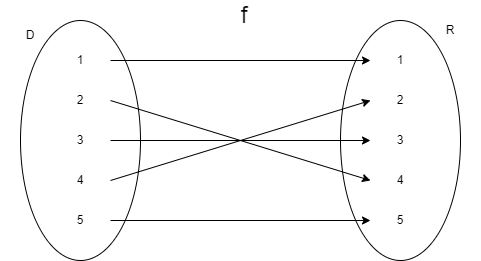
\includegraphics[scale=0.6]{blobs-and-arrows diagram.png}
        \end{figure}

        In the figure above, the name of the function is hung over the main diagram, while the left ellipse denote the set of elements of domain $D$ and the right ellipse denote the range of elements of codomain $R$. The letter $R$ could also be interpreted as the range of $f$.
    \end{example}

    For a discrete function with finitely many inputs, where we will take them as a sequence, it can also be used to represent it efficiently. We just need to have some modification.

    \begin{axiom}
        Let $f:D\to R$ be a function. Let $a_1,a_2,a_3,\dots,a_n$ be a sequence of numbers in $D$ and $b_1,b_2,b_3,\dots, b_n$ be a sequence of numbers in $R$. Suppose $b_1=f(a_1), b_2=f(a_2), \dots , b_n=f(a_n)$ defines the one-to-one correspodence from $D$ to $R$. Then the following blobs-and-arrows diagram describes $f$ formally:

        \begin{figure}[H]
            \centering
            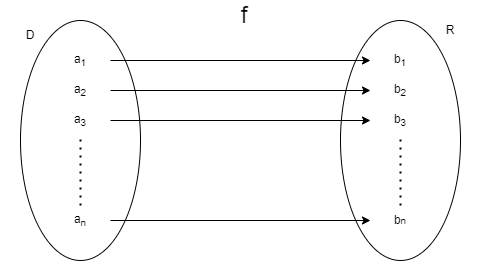
\includegraphics[scale=0.6]{blobs-and-arrows diagram sequence.png}
        \end{figure}
    \end{axiom}

    \begin{exercise}
        Draw the blobs-and-arrows diagram for the following discrete functions:\begin{enumerate}
            \item $f(1)=3, f(2)=6, f(3)=7, f(4)=2, f(5)=3$.
            \item $f(x):=\begin{cases}
                1 &,x=1,2,3,4,5\\
                2 &,x=6,7\\
                3 &,x=8,9,10\\
                4 &,x=11,12,13,14,15\\
                5 &,x=16,17,18,19\\
                6 &,x=20
            \end{cases}$
        \end{enumerate}
    \end{exercise}

    \subsubsection*{The pairing table and xy-coordination}

    To extend our concept of function from discrete version to continuous version, that is, infinitely many numbers can be plugged into the function for calculation, we may need to `fill up' the holes of the domain. 
    
    Let say we have 1 and 2 in the domain $D$, then all the real numbers within 1 and 2 also in $D$. This is the process of \textbf{continuation} or \textbf{extension}, and the whole set of real numbers within 1 and 2 is called the \textbf{interval} between 1 and 2. We can denote the interval by $[1,2]$ if 1 and 2 are included in the meaning, or $(1,2)$ if 1 and 2 are excluded from the meaning. To better distinct the difference between $[1,2]$ and $(1,2)$, we call the previous one the \textbf{closed interval} between 1 and 2, while the latter one the \textbf{open interval} between 1 and 2.

    From this point of view, a real number line is used to represent the concept of any intervals. Let's define the real number line and discuss intervals using a number line.

    \begin{definition}[Real number line]
        A \textbf{real number line} is a straight line with ordered property so that one of its direction is increasing, and the other direction is decreasing.
    \end{definition}

    We usually draw a horizontal real number line for convenience.

    \begin{figure}[H]
        \centering
    \end{figure}

    For the sake of simplicity and connected-understanding of open and closed intervals, we may put the desired parenthesis in the real number line to denote the meaning. Following that a closed interval is in a block-typed while open interval is in a round-typed, we can directly place them on the real number line.

    \begin{example}
        The open interval $(0,1)$.
    \end{example}

    \begin{example}
        The open interval $(-1.5,5.5)$.
    \end{example}

    \begin{example}
        The closed interval $[0.5,1]$.
    \end{example}

    \begin{example}
        The closed interval $[-100,-67]$.
    \end{example}

    \begin{exercise}
        Draw the mentioned interval on the provided real number line with suitable parenthesis.
        \begin{enumerate}
            \item $[0,1]$.
            \item $[\alpha,\beta]$.
            \item $(0,1)$.
            \item $(\alpha,\beta)$.
        \end{enumerate}
    \end{exercise}

    It is of course we could draw it vertically with the same meaning, by indicating upward as positive direction and downward as negative direction. Consider a function $y=f(x)$ defines the relation between $x$ and $y$ coordinate, we can combine two real number lines in an orthogonal way, like a cross, to present the coordination in a sensible way. This is called the \textbf{continuous graph of a function}, or we simply call it the \textit{graph of a function} if there's no ambiguity of what we are discussing.

    In order to draw the graph of a function, we need to figure out the valid pairs of $x$ and $y$ first, so that the points could be addressed correctly for the function. We will make use of a \textbf{pairing table} so that each value of $x$ in the domain is paired with a unique value of $y$ in the co-domain. We will show its use with some examples.

    \begin{example}
        Let $G$ be the graph of $y=x+1$. Then we have the table of testing xy-pair 
        \begin{center}
            \begin{tabular}{|c|c|c|c|c|c|}
                \hline
                $x$&0&1&2&3&4\\
                \hline
                $y=x+1$&1&2&3&4&5\\
                \hline
            \end{tabular}
        \end{center}
        and thus the graph of $G$ be like

        by linking up the points with straight lines.
    \end{example}

    \begin{example}
        Let $G$ be the graph of $y=x^2$. Then we have the table of testing xy-pair 
        \begin{center}
            \begin{tabular}{|c|c|c|c|c|c|}
                \hline
                $x$&-2&-1&0&1&2\\
                \hline
                $y=x^2$&4&1&0&1&4\\
                \hline
            \end{tabular}
        \end{center}
        and thus the graph of $G$ be like

        by linking up the points with straight lines. Moreover, by increasing the points of testing value to, say, 100 or 1000, a see-smoothing curve can be drawn by computer.
        
        It is the continuation of the curve under testing value control.
    \end{example}

    Even higher power polynomial functions can be drawn using this strategy.
    \begin{example}
        Let $G$ be the graph of $y=x^3+2x^2+x-1$. Then we have the table of testing xy-pair 
        \begin{center}
            \begin{tabular}{|c|c|c|c|c|c|}
                \hline
                $x$&0&1&2&3&4\\
                \hline
                $y=x^3+2x^2+x-1$&-1&3&17&47&99\\
                \hline
            \end{tabular}
        \end{center}
        and thus the graph of $G$ be like, with many enough testing points, 

        with the continuation.
    \end{example}

    \begin{exercise}
        Configure the xy-table with testing values in between -3 to 3 and draw a suitable graph for the following functions.\begin{enumerate}
            \item $y=x-3$;
            \item $y=x^2+x+1$;
            \item $y=(x-3)^3+2$.
        \end{enumerate}
        You may also check the graph using WolframAlpha desktop to convince yourself with the plot. Try to conclude the difference between large amount and small amount of points of testing.
    \end{exercise}

    With the xy-coordination of a graph, many features and prediction could be done. We will try to analyze the properties that we could make use of in the next subsection.

    \subsection{Fundamental properties of a graph}

    A graph shows the relationship between two variables, namely the vertical component (in this case, it is the value of $y$) and the horizontal component (respectively, the value of $x$). We will make use of this relationship and consider different situations.

    \subsubsection*{points lying on the graph}

    Let us reverse the sight of plotting a graph of a function. We plot the graph by linking up the points we get from inputting $x$ into the function to get the corresponding value of $y$, so that each point $(x,y)$ describes when the function has the input $x$. We could now see that if a point $(x,y)$ is passed through by a curve then it is the same as the point lies on that curve. We shall say the point $(x,y)$ \textbf{satisfies} the equation $y=f(x)$, since this is the definition of a graph.

    \begin{theorem}
        For any real-valued continuous functions $f$, any coordinates $(x,y)$ lies on the graph $y=f(x)$ if and only if the xy-pair satisfies the equation $y=f(x)$.
    \end{theorem}

    \begin{example}
        For a given function $f(x)=3x+1$, the following are true:\begin{enumerate}
            \item The point $(0,1)$ lies on $y=f(x)$;
            \item The point $(3,10)$ lies on $y=f(x)$;
            \item The point $(-2,1)$ does not lay on $y=f(x)$;
            \item The point $(-10,2)$ does not lay on $y=f(x)$.
        \end{enumerate} 
    \end{example}

    \begin{example}
        For a given function $f(x)=3x^3+2x^2+x+1$, the following are true:\begin{enumerate}
            \item The point $(0,1)$ lies on $y=f(x)$;
            \item The point $(-1,-1)$ lies on $y=f(x)$;
            \item The point $(-2,0)$ does not lay on $y=f(x)$;
            \item The point $(-10,2)$ does not lay on $y=f(x)$.
        \end{enumerate} 
    \end{example}

    \begin{exercise}
        For a given function $f(x)=x^2-1$, show whether the following points are lying on the graph of $y=f(x)$:\begin{enumerate}
            \item The point $(0,1)$;
            \item The point $(-1,0)$;
            \item The point $(-2,3)$;
            \item The set of points $(-t,t^2-1)$ parametrized by the variable $t$.
        \end{enumerate} 
    \end{exercise}

    We may now examine another feature of a graph, namely \textbf{the region of inequality}. In the previous paragraph we find a point satisfying the equation $y=f(x)$ has the same meaning as the point lies on the curve. If we make a small translation of the $y$ coordinate to the upper region separate by the curve, it becomes that all the points have a larger value of $y$ than we could calculate by the function. For that region we will call it the region for $y>f(x)$; Similarly, if we make a small translation of the $y$ coordinate to the lower region, it becomes that all the points in that region have a smaller value of $y$ than we could calculate by the function. For that region, we will call it the region for $y<f(x)$.

    \begin{example}
        For a given function $f(x)=3x+1$, the following are true:\begin{enumerate}
            \item The point $(0,2)$ lies above $y=f(x)$;
            \item The point $(3,9)$ lies below $y=f(x)$;
            \item The point $(-2,1)$ lies above $y=f(x)$;
            \item The point $(-10,-120)$ lies below $y=f(x)$.
        \end{enumerate} 
    \end{example}

    \begin{example}
        For a given function $f(x)=3x^3+2x^2+x+1$, the following are true:\begin{enumerate}
            \item The point $(0,3)$ lies above $y=f(x)$;
            \item The point $(-1,-2)$ lies below $y=f(x)$;
            \item The point $(-2,0)$ lies above $y=f(x)$;
            \item The point $(10,2)$ lies below $y=f(x)$.
        \end{enumerate} 
    \end{example}

    \begin{exercise}
        For a given function $f(x)=x^2-1$, determine the position of the following points with respect to the graph of $y=f(x)$:\begin{enumerate}
            \item The point $(0,9)$;
            \item The point $(-1,-1)$;
            \item The point $(-2,20)$;
            \item The point $(10,10)$.
        \end{enumerate} 
    \end{exercise}

    \subsubsection*{Special intersections: axis intercepts}

    Usually the most important element of a graph is whether it cuts the coordinating axis, namely the y-axis and the x-axis. For practical reason we value them so much and we may give them special names: the y-intercept and the x-intercept.

    \begin{definition}[y-intercept of a graph]
        Given a function $f$, the function has its \textbf{y-intercept} when its cuts the y-axis. In other words, the y-intercept is defined as $$y_0:=f(0)$$ whenever the function is well-defined at $x=0$.
    \end{definition}

    Similarly, we may want the same definition for x-intercept of a graph, however, we do not know whether the inverse function exists or not. This comes to some kind of difficulties to say directly the x-intercept. But still, we can give the possible condition for the discussion.

    \begin{definition}[x-intercept of a graph]
        Given a function $f$, the function has its \textbf{x-intercept} when its cuts the x-axis. In other words, the x-intercept is defined as the roots of $$0=f(x)$$ whenever the given equation is solvable.
    \end{definition}

    We will be familiar with them with some valid examples.

    \begin{example}
        For the graph of the function $f(x):=x+1$, we have:\begin{itemize}
            \item y-intercept: $y_0=0+1=1$;
            \item x-intercept: Set $0=x+1$, then $x_0=-1$ is the root to the given equation, which is the x-intercept of the function.
        \end{itemize}
    \end{example}

    \begin{example}
        For the graph of the function $f(x):=x^2-1$, we have:\begin{itemize}
            \item y-intercept: $y_0=0^2-1=-1$;
            \item x-intercept: Set $0=x^2-1$, then $x_1=-1$ or $x_2=1$ are the roots to the given equation, which are the x-intercepts of the function.
        \end{itemize}
    \end{example}

    \begin{example}
        For the graph of the function $f(x):=x^2+1$, we have:\begin{itemize}
            \item y-intercept: $y_0=0^2+1=1$;
            \item x-intercept: Set $0=x^2+1$, which has no real solution. Then the graph of the function has no x-intercepts.
        \end{itemize}
    \end{example}

    We see a function has its y-intercept most of the time, but not the same case for x-intercepts. It could have either no x-intercepts, only 1 x-intercept, or more than one x-intercept. It is a consequence of the fundamental theorem of algebra, but we will dig deeper in the future to discuss simple cases we could.

    As long as we could plot not only the xy-coordinate but we could pair up something weird, where they could be different functions say $v(y)$ and $u(x)$, the graphs could no longer talked about y-intercept or x-intercept - they are not exactly about x and y! Hence, we turned the naming into something general: we plot the graph by vertical axis and horizontal axis, so let us call them the \textbf{vertical intercept} and the \textbf{horizontal intercept} respectively.

    \subsection{Solving equations using graphs of functions}

    \subsubsection*{Homogeneous equations}

    \subsubsection*{Non-homogeneous equations}

    \subsubsection*{Simultaneous equations}

    \subsection{Transformation of functions}

    \subsubsection*{Translation}

    \subsubsection*{Dilation}

    \subsection{Challenging questions}

    \newpage

    \section{Trigonometric functions}

    A right-angled triangle is usually a pure triangle we want to study the beauty of geometry. In this section, we are going to examine the usage of trigonometric functions as far as we could.

    \subsection{Why are we calling it `trigonometry' ?}

    The word 'trigonometry' can be divided into two parts - `trigono-' and `-metry'. The word `trigono-' comes from the word `trigonal', meaning `the things of trigon'. What trigon means is a triangle: in English, the word `tri-' means the number 3, and what counts to 3 can be named `tri-' things, like tripoid, triangle, tricycle, trisep, etc. So a trigon is equal to a triangle, just a difference in perspective: one tries to describe the number of vertices in a polygon, while one makes a point to number of angles in it. Another word `-metry' comes from the word `metric', which means `the method of comparison'. In complete word, `trigonometry' means `the method of comparison of triangle'. Therefore, when we learn trigonometry, we will compare many attributes: the length of sides in one triangle, the shapes and sizes of different triangles.

    \subsection{The relation of sides of triangle}

    We shall first declare what is a triangle, how it forms and what is special about it.

    \subsubsection*{Triangle inequality and Pythagoras theorem}

    Given a triangle, if we could draw it on a plane, we must have it with following axiomatic structures:\begin{itemize}
        \item There are 3 vertices in a triangle.
        \item There are 3 edges connecting 3 vertices.
        \item Given a vertex and its adjacent edges, an angle is formed. There are 3 angles in total.
    \end{itemize}

    To emphasize the structure inheriting 3 angles, we call it a \textbf{triangle}, with the prefix \textit{tri-} standing for the number 3.

    We shall immediate find a property of any given triangle that any edge in a triangle must be shorter than the sum of length of the other two edges. Here we call it \textbf{the triangle inequality}.

    \begin{axiom}[Triangle inequality]
        Let $a,b,c$ be some positive numbers. If they denote the side lengths of a triangle, then we have the following inequalities:\begin{itemize}
            \item $a+b\geq c$;
            \item $a+c\geq b$;
            \item $b+c\geq a$.
        \end{itemize}
    \end{axiom}

    We shall take them as axioms, since we do not need to dig too deep to the roots of such geometric constructions. We shall take it to be true with our intuition.

    \begin{theorem}[Pythagoras theorem]
        Let $a,b,c$ be positive numbers. Let $a,b$ be the adjacent sides of a right-angled triangle and $c$ be the hypotenuse of the right-angled triangle. Then $$a^2+b^2=c^2$$
    \end{theorem}

    \begin{corollary}
        The following holds for a right-angled triangle with adjacent sides $a,b$ and hypotenuse $c$.
        \begin{itemize}
            \item $a<c$;
            \item $b<c$.
        \end{itemize}
    \end{corollary}

    \subsubsection*{The Sine function}

    Historically, the sine function is defined for the relation between the opposite side of a given acute angle in a triangle and the hypotenuse of the triangle.

    \begin{definition}[The Sine function]
        Let $a,b,c$ be sides of a given right-angled triangle and $\theta$ be an acute angle inside the triangle as shown.

        Then the \textbf{sine function of $\theta$}, $\sin{\theta}$, is defined by $$\sin{\theta}:=\frac{a}{c}$$
    \end{definition}

    In some sense, we call the side $a$ the opposite side of $\theta$ and $c$ the hypotenuse. We so shorthand opposite side by 'o' and hypotenuse by 'h'. This produces a well known memorization technique of the relation described by sine function, read as 'soh' relation.

    \begin{theorem}
        The range of the sine function in a right-angled triangle is constrained to be $$0<\sin{\theta}<1$$
    \end{theorem}

    \begin{proof}
        By definition, $a<c$, so $\frac{a}{c}<1$; at the same time, $a>0$ and $c>0$, hence $\frac{a}{c}>0$.
    \end{proof}

    \subsubsection*{The Cosine function}

    The cosine function is defined for the relation between the adjacent side of a given acute angle in a triangle and the hypotenuse of the triangle.

    \begin{definition}[The Cosine function]
        Let $a,b,c$ be sides of a given right-angled triangle and $\theta$ be an acute angle inside the triangle as shown.

        Then the \textbf{cosine function of $\theta$}, $\cos{\theta}$, is defined by $$\cos{\theta}:=\frac{b}{c}$$
    \end{definition}

    In some sense, we call the side $b$ the adjacent side of $\theta$ and $c$ the hypotenuse. We so shorthand adjacent side by 'a' and hypotenuse by 'h'. This produces a well known memorization technique of the relation described by cosine function, read as 'cah' relation.

    \begin{theorem}
        The range of the sine function in a right-angled triangle is constrained to be $$0<\cos{\theta}<1$$
    \end{theorem}

    \begin{proof}
        By definition, $b<c$, so $\frac{b}{c}<1$; at the same time, $b>0$ and $c>0$, hence $\frac{b}{c}>0$.
    \end{proof}

    \subsubsection*{The tangent function}

    The tangent function is defined for the relation between the opposite side and the adjacent side of a given acute angle in a triangle.

    \begin{definition}[The Tangent function]
        Let $a,b,c$ be sides of a given right-angled triangle and $\theta$ be an acute angle inside the triangle as shown.

        Then the \textbf{tangent function of $\theta$}, $\tan{\theta}$, is defined by $$\tan{\theta}:=\frac{a}{b}$$
    \end{definition}

    In some sense, we call the side $a$ the opposite side of $\theta$ and $b$ the opposite side of $\theta$. We so shorthand opposite side by 'o' and adjacent side by 'a'. This produces a well known memorization technique of the relation described by tangent function, read as 'toa' relation.

    \begin{theorem}
        The range of the sine function in a right-angled triangle is constrained to be $$0<\sin{\theta}$$
    \end{theorem}

    \begin{proof}
        By definition, $a>0$ and $b>0$, hence $\frac{a}{b}>0$.
    \end{proof}

    \subsubsection*{Fundamental identities for trigonometric functions}

    \begin{theorem}
        $\sin(90^\circ - \theta)=\cos{\theta}$
    \end{theorem}

    \begin{proof}
        Suppose $a,b,c$ be the opposite side, the adjecent side and the hypotenuse to the acute angle $\theta$ in a right-angled triangle respectively. Note that by the law of angle sum of triangle, if we denote the remaining angle other than $\theta$ and $90^\circ$ by $\phi$, we get $\phi = 90^\circ - \theta$. Then \begin{align*}
            \sin(90^\circ - \theta) &= \sin{\phi}\\
            &= \frac{b}{c}\\
            &= \cos{\theta}
        \end{align*}
    \end{proof}

    \begin{corollary}
        $\cos(90^\circ - \theta)=\cos{\theta}$
    \end{corollary}

    \begin{theorem}
        $\sin^2{\theta}+\cos^2{\theta}=1$.
    \end{theorem}

    \begin{proof}
        Suppose $a,b,c$ be the opposite side, the adjecent side and the hypotenuse to the acute angle $\theta$ in a right-angled triangle respectively. Then \begin{align*}
            \sin^2{\theta}+\cos^2{\theta}&=(\frac{a}{c})^2+(\frac{b}{c})^2\\
            &=\frac{a^2}{c^2}+\frac{b^2}{c^2}\\
            &=\frac{a^2+b^2}{c^2}\\
            &=\frac{c^2}{c^2}=1
        \end{align*}
    \end{proof}

    \begin{theorem}
        $\tan{\theta}=\dfrac{\sin{\theta}}{\cos{\theta}}$.
    \end{theorem}

    \begin{proof}
        Suppose $a,b,c$ be the opposite side, the adjecent side and the hypotenuse to the acute angle $\theta$ in a right-angled triangle respectively. Then \begin{align*}
            \frac{\sin{\theta}}{\cos{\theta}}&=\sin{\theta}/ \cos{\theta}\\
            &=\frac{a}{c}/ \frac{b}{c}\\
            &=\frac{a}{c}\cdot \frac{c}{b}\\
            &=\frac{a}{b}\\
            &=\tan{\theta}
        \end{align*}
    \end{proof}

    \begin{example}
        Simplify the expression $\dfrac{[\sin(90^\circ - \theta) - \cos(90^\circ - \theta)]^2}{1-(\tan{\theta})(2\cos^2{\theta})}$.

        \textit{ Sol. }By proved theorem, we have \begin{align*}
            \frac{[\sin(90^\circ - \theta) - \cos(90^\circ - \theta)]^2}{1-(\tan{\theta})(2\cos^2{\theta})} &= \frac{(\cos{\theta}-\sin{\theta})^2}{1-(\frac{\sin{\theta}}{\cos{\theta}})(\cos^2{\theta})}\\
            &= \frac{\cos^2{\theta}-2\sin{\theta}\cos{\theta}+\sin^2{\theta}}{1-2\sin{\theta}\cos{\theta}}\\
            &= \frac{1-2\sin{\theta}\cos{\theta}}{1-2\sin{\theta}\cos{\theta}}\\
            &= 1
        \end{align*}
    \end{example}

    \subsection{The compound angle formulae}

    Someone might be interested in computing compound angle formulae, which are important in developing different results of trigonometric relations. We will assume that $\alpha$ and $\beta$ are both acute angles, so that all the results could be applied to whenever $0<\alpha+\beta<180^\circ$.

    Consider the following sector with radius 1:
    \begin{figure}[H]
        \centering
        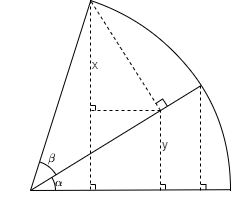
\includegraphics[scale=0.8]{ab.png}
    \end{figure}

    \begin{theorem}
        $\sin(\alpha+\beta)=\sin{\alpha}\cos{\beta}+\sin{\beta}\cos{\alpha}$.
    \end{theorem}

    \begin{proof}
        Referring to the figure, we have $\sin(\alpha+\beta)=x+y$.
        
        On the other hand, we have $$\begin{cases}
            x=\sin{\beta}\cos{\alpha}\\y=\cos{\beta}\sin{\alpha}
        \end{cases}$$ Therefore, $\sin(\alpha+\beta)=\sin{\alpha}\cos{\beta}+\sin{\beta}\cos{\alpha}$.
    \end{proof}

    For now we have the result for $\sin(\alpha+\beta)$. Then the remaining results could be proven under substitution of variables:
    
    \begin{theorem}
        $\sin(\alpha-\beta)=\sin{\alpha}\cos{\beta}-\sin{\beta}\cos{\alpha}$.
    \end{theorem}

    \begin{proof}
        \begin{align*}
            \sin(\alpha-\beta)&=\sin(\alpha+(-\beta))\\&=\sin{\alpha}\cos(-\beta)+\sin(-\beta)\cos{\alpha}\\&=\sin{\alpha}\cos{\beta}-\sin{\beta}\cos{\alpha}
        \end{align*}
    \end{proof}

    \begin{theorem}
        $\cos(\alpha+\beta)=\cos{\alpha}\cos{\beta}-\sin{\alpha}\sin{\beta}$.
    \end{theorem}

    \begin{proof}
        \begin{align*}
            \cos(\alpha+\beta)&=\sin(\frac{\pi}{2}-(\alpha+\beta))\\&=\sin(\frac{\pi}{2}-\alpha)\cos(-\beta)+\sin(-\beta)\cos(\frac{\pi}{2}-\alpha)\\&=\cos{\alpha}\cos{\beta}-\sin{\alpha}\sin{\beta}
        \end{align*}
    \end{proof}

    \begin{theorem}
        $\cos(\alpha-\beta)=\cos{\alpha}\cos{\beta}+\sin{\alpha}\sin{\beta}$.
    \end{theorem}

    \begin{proof}
        \begin{align*}
            \cos(\alpha-\beta)&=\cos(\alpha+(-\beta))\\&=\cos{\alpha}\cos(-\beta)-\sin{\alpha}\sin(-\beta)\\&=\cos{\alpha}\cos{\beta}+\sin{\alpha}\sin{\beta}
        \end{align*}
    \end{proof}

    \begin{theorem}
        $\tan(\alpha+\beta)=\frac{\tan{\alpha}+\tan{\beta}}{1-\tan{\alpha}\tan{\beta}}$.
    \end{theorem}

    \begin{proof}
        \begin{align*}
            \tan(\alpha+\beta)&=\frac{\sin(\alpha+\beta)}{\cos(\alpha+\beta)}\\&=\frac{\sin{\alpha}\cos{\beta}+\sin{\beta}\cos{\alpha}}{\cos{\alpha}\cos{\beta}-\sin{\alpha}\sin{\beta}}\\&=\frac{\frac{\sin{\alpha}}{\cos{\alpha}}+\frac{\sin{\beta}}{\cos{\beta}}}{1-\frac{\sin{\alpha}}{\cos{\alpha}}\frac{\sin{\beta}}{\cos{\beta}}}\\&=\frac{\tan{\alpha}+\tan{\beta}}{1-\tan{\alpha}\tan{\beta}}
        \end{align*}
    \end{proof}

    \begin{theorem}
        $\tan(\alpha-\beta)=\frac{\tan{\alpha}-\tan{\beta}}{1+\tan{\alpha}\tan{\beta}}$
    \end{theorem}

    \begin{proof}
        \begin{align*}
            \tan(\alpha-\beta)&=\frac{\tan{\alpha}+\tan(-\beta)}{1-\tan{\alpha}\tan(-\beta)}\\
            &=\frac{\tan{\alpha}-\tan{\beta}}{1+\tan{\alpha}\tan{\beta}}
        \end{align*}
    \end{proof}

    All the results shown are based on $\alpha+\beta<90^\circ$, so the case where $\alpha+\beta>90^\circ$ are left to students.

    \subsection{The trigonometric laws}

    To understand the trigonometric functions better, we will try to extend the meaning of the trigonometric functions. The first step is to construct some laws with them so that the meaning could be seen.

    In our discussion, we will look at two different triangles: one with acute angles only, while another with one obtuse angle. We will refer to the following triangles by $T_1$ and $T_2$ at anytime.

    \begin{figure}[H]
        \centering
        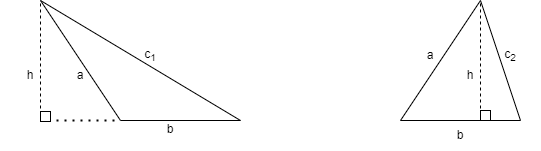
\includegraphics[scale=0.8]{triangles.png}
        \caption{$T_1$ (left) and $T_2$ (right)}
    \end{figure}

    In convenience, we will denote the angle opposite to $c_i$ to be $\gamma_i$. $\alpha$ to $a$ and $\beta$ to $b$.

    \subsubsection*{The area formula of a triangle}

    Consider the area of $T_1$ and $T_2$, if we are taken their height to be the same, we will have the following interesting results:

    Consider the area of $T_2$, we have $h=a\sin(\gamma_2)$, so its area is $$\frac{1}{2}ab\sin(\gamma_2)$$

    Consider the area of $T_1$, we have $h=a\sin(180^\circ - \gamma_1)$. The value of $\sin(180^\circ - \gamma_1)$ can be obtained by consiering \begin{align*}
        \gamma_1 &= 180^\circ - \alpha - \beta\\
        \sin{\gamma_1}&=\sin(180^\circ - \alpha - \beta)\\
        &=\sin((90^\circ - \alpha) + (90^\circ - \beta))\\
        &=\sin(90^\circ - \alpha)\cos(90^\circ - \beta)+ \cos(90^\circ - \alpha)\sin(90^\circ - \beta)\\
        &=\cos{\alpha}\sin{\beta}+\sin{\alpha}\cos{\beta}\\
        &=\sin(\alpha+\beta)\\
        &=\sin(180^\circ - \gamma_1)
    \end{align*}

    Hence, we have its area to be \begin{align*}
        \frac{1}{2}ab\sin(180^\circ - \gamma_1)&=\frac{1}{2}ab\sin(\gamma_1)
    \end{align*}

    In conclusion, the area of a triangle with given angle $\theta$ and adjacent sides can be computed as 

    \begin{theorem}
        Given a triangle with a given angle $\theta$ in which $0\leq \theta\leq 180^\circ$ and corresponding adjacent sides of length $a$ and $b$, the area of the triangle is $$\frac{1}{2}ab\sin{\theta}$$
    \end{theorem}

    \subsubsection*{The Sine Law}

    Our first law in discussion of trigonometric function is the \textbf{sine law} - the law inheriting the charateristics of sine function.

    \begin{theorem}[Sine Law]
        $\displaystyle \frac{a}{\sin{\alpha}}=\frac{b}{\sin{\beta}}=\frac{c_i}{\sin{\gamma_i}}$.
    \end{theorem}

    \begin{proof}[Proof by extended right-angle triangle]
        We first complete the case in $T_2$. It is not hard to see that \begin{align*}
            c_2\sin{\alpha}&=a\sin{\gamma_2}\\
            \frac{c_2}{\sin{\gamma_2}}&=\frac{a}{\sin{\alpha}}
        \end{align*}
        By rotation, similar results can be proven for other equality. We are done in the case of $T_2$.

        We then look at the case of $T_1$. As in area computation, we shall see that \begin{align*}
            \sin{\gamma_1}&=\sin(180^\circ - \gamma_1)
        \end{align*}
        Then \begin{align*}
            c_1\sin{\alpha}&=a\sin(180^\circ - \gamma_1)\\
            \frac{c_1}{\sin{\gamma_1}}&=\frac{a}{\sin{\alpha}}
        \end{align*}
    \end{proof}

    \begin{proof}[Proof by area formula]
        Consider the area of the triangle, we obtain the following equality:

        $$\frac{1}{2}ab\sin{\gamma}=\frac{1}{2}bc\sin{\alpha}=\frac{1}{2}ac\sin{\beta}$$

        which yields the following result when dividing each expression by $\dfrac{abc}{2}$:

        $$\frac{\sin{\gamma}}{c}=\frac{\sin{\alpha}}{a}=\frac{\sin{\beta}}{b}$$
    \end{proof}

    The law connects an angle with its opposite sides by the ratio of sine function. This is a good perspective to apply the formula to solve any triangle with given two sides and an angle.

    \begin{example}
        Suppose a triangle $\triangle ABC$ with $AB=3, AC=5, \angle B = 60^\circ$. Then it is not hard to see \begin{align*}
            \frac{AC}{\sin{\angle B}}&=\frac{AB}{\sin{\angle C}}=\frac{BC}{\sin{\angle A}}\\
            \sin{\angle C}&=\frac{3\sin{60^\circ}}{5}\\
            &=\frac{3\sqrt{3}}{10}\\
            \sin{\angle A}&=\sin{\angle B}\cos{\angle C}+\sin{\angle C}\cos{\angle B}\\
            &=\frac{\sqrt{3}}{2}\cdot \frac{\sqrt{73}}{10}+\frac{3\sqrt{3}}{10}\cdot \frac{1}{2}\\
            &=\frac{\sqrt{219}+3\sqrt{3}}{20}\\
            BC&=\frac{10\sqrt{3}}{3}\cdot\frac{\sqrt{219}+3\sqrt{3}}{20}\\
            &=\frac{3+\sqrt{73}}{2}
        \end{align*}
    \end{example}

    \begin{remark}
        It is the usual sine function when one of the angle becomes $90^\circ$.
    \end{remark}

    \subsubsection*{The Cosine Law}

    The second law in trigonometry to be discussed will be the \textbf{cosine law} - the law inheriting cosine function.

    \begin{theorem}[Cosine Law]
        The following formulae holds:\begin{itemize}
            \item $c^2=a^2+b^2-2ab\cos{\gamma} \iff \cos{\gamma}=\dfrac{a^2+b^2-c^2}{2ab}$.
            \item $b^2=a^2+c^2-2ac\cos{\beta} \iff \cos{\beta}=\dfrac{a^2+c^2-b^2}{2ac}$.
            \item $a^2=b^2+c^2-2bc\cos{\alpha} \iff \cos{\alpha}=\dfrac{b^2+c^2-a^2}{2bc}$.
        \end{itemize}
    \end{theorem}

    \begin{proof}[Standard proof]
        We first see the case in $T_2$. It is not hard to see if we partition $b$ into $x+y$ according to their order, we could construct the relations \begin{align*}
            \begin{cases}
                x+y&=b\\
                a^2-x^2&=h^2=c_2^2-y^2\\
                x&=a\cos{\gamma_2}
            \end{cases}
            &\implies \begin{cases}
                a^2-x^2&=c_2^2-(b-x)^2\\
                x&=a\cos{\gamma_2}
            \end{cases}\\
            &\implies \begin{cases}
                a^2+b^2-2bx&=c_2^2\\
                x&=a\cos{\gamma_2}
            \end{cases}\\
            &\implies c_2^2=a^2+b^2-2ab\cos{\gamma_2}
        \end{align*}

        On the other hand, for $T_1$, we have to tackle particularly the obtused angle case. Note that if $T_1$ is divided into two right-angled triangle, then $\gamma_1$ can be divided into $\theta_1+\theta_2$. It is equivalent to say \begin{align*}
            \cos{\gamma_1}&=\cos{\theta_1}\cos{\theta_2}-\sin{\theta_1}\sin{\theta_2}\\
            &=\sin(90^\circ - \theta_1)\sin(90^\circ - \theta_2) - \cos(90^\circ - \theta_1)\cos(90^\circ - \theta_2)\\
            &=-\cos(180^\circ -\gamma_1)
        \end{align*}
        Therefore, we pick to consider $x=a\cos(180^\circ - \gamma_1)$, then \begin{align*}
            c_1^2 - (b+x)^2 &= a^2-x^2\\
            c_1^2 - b^2 - 2bx &= a^2\\
            c_1^2 &= a^2 + b^2 + 2ab\cos(180^\circ - \gamma_1)\\
            c_1^2 &= a^2 + b^2 - 2ab\cos{\gamma_1}
        \end{align*}
        This concludes that in any case, the cosine law holds.
    \end{proof}

    The best part of cosine law is that it generalizes the Pythagoras theorem to aritrary triangles. It is also more applicable than Sine law to different situations.

    \begin{example}
        Refer to the same example in sine law. We can now directly find the length of $BC$.

        \begin{align*}
            AC^2 &= AB^2 + BC^2 - 2\cdot AB\cdot BC\cos{\angle B}\\
            5^2 &= 3^2 + BC^2 - 2\cdot 3\cdot BC\cos{60^\circ}\\
            0 &= BC^2 - 3BC - 16
        \end{align*}

        Shall we learn to solve quadratic equations, the solution to the equation is $\dfrac{3\pm \sqrt{3^2-4(-16)}}{2}=\dfrac{3\pm \sqrt{73}}{2}$. Since $\sqrt{73}>3$, we need $BC>0$, so $BC=\dfrac{3+\sqrt{73}}{2}$.
    \end{example}

    \subsubsection*{The Tangent Law}

    It is the third law in trigonometry, which uses less but still understandable to write down. It is the \textbf{tangent law} - a law inheriting tangent function as its argument.

    \begin{theorem}[Tangent Law]
        The following formulae holds:\begin{itemize}
            \item $\dfrac{a-b}{a+b}=\dfrac{\tan{\frac{\alpha-\beta}{2}}}{\tan{\frac{\alpha+\beta}{2}}}$.
            \item $\dfrac{b-c}{b+c}=\dfrac{\tan{\frac{\beta-\gamma}{2}}}{\tan{\frac{\beta+\gamma}{2}}}$.
            \item $\dfrac{c-a}{c+a}=\dfrac{\tan{\frac{\gamma-\alpha}{2}}}{\tan{\frac{\gamma+\alpha}{2}}}$.
        \end{itemize}
    \end{theorem}

    \begin{proof}[Algebraic proof]
        Consider $\dfrac{\tan{\frac{\alpha-\beta}{2}}}{\tan{\frac{\alpha+\beta}{2}}}$. Denote $t_\alpha = \tan{\frac{\alpha}{2}}$ and $t_\beta = \tan{\frac{\beta}{2}}$.

        \begin{align*}
            \frac{\tan{\frac{\alpha-\beta}{2}}}{\tan{\frac{\alpha+\beta}{2}}}&=\frac{\tan{\frac{\alpha}{2}}-\tan{\frac{\beta}{2}}}{1+\tan{\frac{\alpha}{2}}\tan{\frac{\beta}{2}}}\frac{1-\tan{\frac{\alpha}{2}}\tan{\frac{\beta}{2}}}{\tan{\frac{\alpha}{2}}+\tan{\frac{\beta}{2}}}\\
            &=\frac{t_\alpha - t_\beta - t_\alpha^2t_\beta+t_\alpha t_\beta^2}{t_\alpha + t_\beta + t_\alpha^2t_\beta+t_\alpha t_\beta^2}\\
            &=\frac{t_\alpha(\sec^2{\frac{\beta}{2}})-t_\beta(\sec^2{\frac{\alpha}{2}})}{t_\alpha(\sec^2{\frac{\beta}{2}})+t_\beta(\sec^2{\frac{\alpha}{2}})}\\
            &=\frac{t_\alpha(\cos^2{\frac{\alpha}{2}})-t_\beta(\cos^2{\frac{\beta}{2}})}{t_\alpha(\cos^2{\frac{\alpha}{2}})+t_\beta(\cos^2{\frac{\beta}{2}})}\\
            &=\frac{\sin{\alpha}-\sin{\beta}}{\sin{\alpha}+\sin{\beta}}\\
            &=\frac{ab\sin{\alpha}-ab\sin{\beta}}{ab\sin{\alpha}+ab\sin{\beta}}\\
            &=\frac{a-b}{a+b}
        \end{align*}
    \end{proof}

    The tangent law relates two angles with two corresponing opposite sides. The application makes an agreement with the sine law, however, without advantages to apply the tangent law because of its complexity. We just do it a favor to learn a complete view to all three trigonometric functions.

    In advance, let's introduce one more result related to the tangent law to close this extra section.

    \begin{theorem}[Mollweide's Equations]
        The following holds:\begin{align}
            \frac{a-b}{c}&=\frac{\sin{\frac{\alpha-\beta}{2}}}{\cos{\frac{\gamma}{2}}}\\
            \frac{a+b}{c}&=\frac{\cos{\frac{\alpha-\beta}{2}}}{\sin{\frac{\gamma}{2}}}
        \end{align}
    \end{theorem}

    \begin{proof}
        As $\alpha,\beta,\gamma$ represents 3 angles in a triangle, their sum agrees with $\alpha+\beta+\gamma=180^\circ$, therefore $\frac{\gamma}{2}=90^\circ - \frac{\alpha+\beta}{2}$. We have the equality \begin{align*}
            \tan{\frac{\alpha+\beta}{2}}&=\frac{1}{\tan{\frac{\gamma}{2}}}
        \end{align*}
        By proved result on the Tangent Law:\begin{align*}
            \frac{a-b}{a+b}&=\frac{\tan{\frac{\alpha-\beta}{2}}}{\tan{\frac{\alpha+\beta}{2}}}\\
            &=\frac{\sin{\frac{\alpha-\beta}{2}}}{\sin{\frac{\alpha+\beta}{2}}}\frac{\cos{\frac{\alpha+\beta}{2}}}{\cos{\frac{\alpha-\beta}{2}}}\\
            &=\frac{\sin{\frac{\alpha-\beta}{2}}}{\cos{\frac{\gamma}{2}}}\frac{\sin{\frac{\gamma}{2}}}{\cos{\frac{\alpha-\beta}{2}}}\\
            &=\frac{\sin{\frac{\alpha-\beta}{2}}}{\cos{\frac{\gamma}{2}}}\frac{2\sin{\frac{\gamma}{2}}\cos{\frac{\gamma}{2}}}{2\cos{\frac{\alpha-\beta}{2}}\cos{\frac{\gamma}{2}}}\\
            &=\frac{\sin{\frac{\alpha-\beta}{2}}}{\cos{\frac{\gamma}{2}}}\frac{\sin{\gamma}}{\sin{\alpha}+\sin{\beta}}\\
            &=\frac{\sin{\frac{\alpha-\beta}{2}}}{\cos{\frac{\gamma}{2}}}\frac{c}{a+b}\\
            \frac{a-b}{c}&=\frac{\sin{\frac{\alpha-\beta}{2}}}{\cos{\frac{\gamma}{2}}}
        \end{align*}
        This proves the first equation.

        For the second equation, consider \begin{align*}
            \frac{a+b}{c}&=\frac{a+b}{a-b}\cdot \frac{a-b}{c}\\
            &=\frac{\tan{\frac{\alpha+\beta}{2}}}{\tan{\frac{\alpha-\beta}{2}}}\frac{\sin{\frac{\alpha-\beta}{2}}}{\cos{\frac{\gamma}{2}}}\\
            &=\frac{\cos{\frac{\alpha-\beta}{2}}}{\sin{\frac{\gamma}{2}}}
        \end{align*}
        Then the Mollweide's equations are proved.
    \end{proof}

    \subsubsection*{Heron's formula}

    In order to compute formula from all perspective, we now look at a well-known formula for computing area of an arbitrary triangle using side length only. This is the Heron's formula.

    \begin{theorem}[Heron's formula]
        Let $a,b,c$ be the side length of 3 sides of a triangle. Then the area of the triangle is computed by $$\sqrt{s(s-a)(s-b)(s-c)}$$where $s=\dfrac{a+b+c}{2}$.
    \end{theorem}

    \begin{proof}[Geometric proof of Heron's formula]
        Let $r$ be the radius of the inscribe circle. Then the area of the triangle can be computed by $$\frac{ra+rb+rc}{2}=rs$$ where $s=\frac{a+b+c}{2}$. 

        \begin{figure}[H]
            \centering
            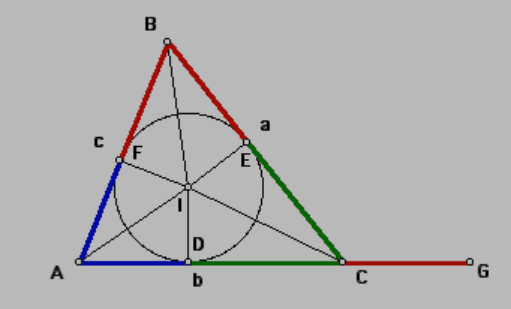
\includegraphics[scale=0.8]{heron.png}
            \caption{Reference: http://jwilson.coe.uga.edu/EMT668/EMAT6680.2000/Umberger/\\MATH7200/HeronFormulaProject/GeometricProof/geoproof.html}
        \end{figure}

        The following steps will try to resolve $rs$ from other perspective. Here we orientate the side $AC$ to be the base of the triangle (parallel to horizon), and extend the segment to $G$ as in the figure. The area becomes $r\cdot AG$.

        Next we adjoin the figure with a line from $I$ so that $\angle AIJ = 90^\circ$ as follows.

        \begin{figure}[H]
            \centering
            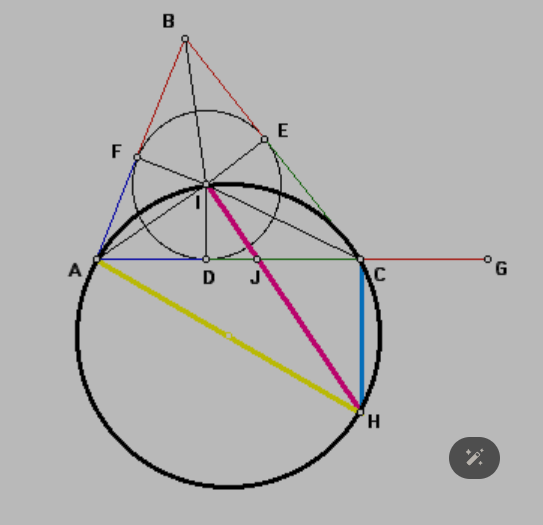
\includegraphics[scale=0.8]{heron_circle.png}
            \caption{Reference: http://jwilson.coe.uga.edu/EMT668/EMAT6680.2000/Umberger/\\MATH7200/HeronFormulaProject/GeometricProof/geoproof.html}
        \end{figure}

        We try to figure out some similar triangles.\begin{align*}
            \angle AHC + \angle AIC &= 180^\circ &(concyclic, \angle \, supp.)\\
            \angle BIE + \angle AIC &= 180^\circ &(\angle s\, at\, a\, pt.)\\
            \therefore \angle AHC &= \angle BIE\\
            \angle BEI = \angle ACH &= 90^\circ &(By \, construction)\\
            \therefore \triangle ACH &\sim \triangle BEI
        \end{align*}

        On the other hand, it is not hard to see that \begin{align*}
            \triangle IDJ &\sim \triangle HCJ
        \end{align*}

        Then the following relation holds:\begin{align*}
            \frac{AC}{CH}&=\frac{BE}{IE}&(\triangle ACH \sim \triangle BEI)\\
            \frac{AC}{CG}&=\frac{CH}{ID}&(BE=CG,IE=ID)\\
            &=\frac{CJ}{DJ}&(\triangle IDJ \sim \triangle HCJ)\\
            \frac{AG}{CG}&=\frac{CD}{DJ}&(+1\, on\, both\, sides)\\
            AG\cdot ID&=\frac{CD}{DJ}CG\cdot ID\\
            &=CD\cdot CG\cdot \frac{AD}{ID}&(\frac{ID}{DJ}=\frac{AD}{ID},\triangle ADI\sim\triangle IDJ)\\
            &=CD\cdot CG\cdot \frac{AD\cdot AG}{ID\cdot AG}\\
            AG\cdot ID&=\sqrt{AD\cdot DC\cdot CG\cdot AG}&(rearrangement)
        \end{align*}

        Which, the area of $\triangle ABC$ is exactly $$AG\cdot ID=\sqrt{AD\cdot DC\cdot CG\cdot AG}$$ and the proof is done.
    \end{proof}

    We have also the algebraic proof of heron's formula which is much sensible.

    \begin{proof}[Algebraic proof of Heron's formula]
        Consider the sine law and cosine law where we have proven to be true in any case. We have the area formula $$A=\frac{1}{2}ab\sin{\gamma}$$ and thus if we do a little trick, square it, we have \begin{align*}
            A^2&=\frac{1}{4}a^2b^2\sin^2{\gamma}\\
            &=\frac{1}{4}a^2b^2(1-\cos^2{\gamma})\\
            &=\frac{1}{4}a^2b^2(1-(\frac{a^2+b^2-c^2}{2ab})^2)\\
            &=\frac{1}{4}a^2b^2(1+\frac{a^2+b^2-c^2}{2ab})(1-\frac{a^2+b^2-c^2}{2ab})\\
            &=\frac{1}{16}(a^2+2ab+b^2-c^2)(c^2-a^2+2ab-b^2)\\
            &=\frac{1}{16}[(a+b)^2-c^2][c^2-(a-b)^2]\\
            &=\frac{1}{16}(a+b+c)(a+b-c)(-a+b+c)(a-b+c)\\
            &=s(s-a)(s-b)(s-c)
        \end{align*}
        Thus, by the positivity of area, we have $$A=\sqrt{s(s-a)(s-b)(s-c)}$$ where $s=\dfrac{a+b+c}{2}$
    \end{proof}

    \begin{example}
        Let $\triangle ABC$ be with sides $7,10,13$. Define $s=\dfrac{7+10+13}{2}=15$. Then the area of the triangle is $$S_{\triangle ABC}=\sqrt{15(15-7)(15-10)(15-13)}=\sqrt{1200}=20\sqrt{3}$$
    \end{example}

    \begin{exercise}
        Compute the area of $\triangle ABC$ if the side lengths are:\begin{enumerate}
            \item 1,2,3.
            \item 3,4,5.
            \item 2,6,7.
            \item 13,15,17.
            \item 9,9,6.
        \end{enumerate}
    \end{exercise}
    \subsection{Extending trigonometric functions to describing circles}

    Trigonometric functions are not bounded by a triangle. In fact, if we want to, and trust to, extend trigonometric functions to any degree, we could still give a definition.

    \subsubsection*{The relation between rectangular coordinates and polar coordinates}

    Let us recall the definitions of coordinate systems and their notations.

    \begin{definition}[Rectangular coordinates]
        A rectangular coordinates is a pair of numbers determining the position with respect to a pair of orthogonal axes, which is also called the rectangular coordinates plane.
    \end{definition}

    \begin{example}
        The positions $(1,2), (3,-2), (-4,0)$ are shown in the following rectangular coordinates plane.
        
        \begin{figure}[H]
            \centering
            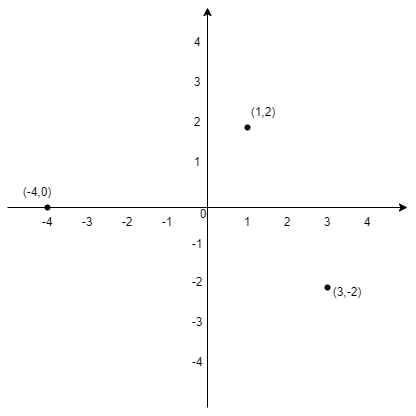
\includegraphics[scale=0.8]{rectangular coordinates.png}
        \end{figure}

        The coordinates are written in an ordered pair with horizontal position first then followed by vertical position.
    \end{example}

    It is important to note and remember that coordinates must be written in a certain order - horzontal position first, then vertical position. Otherwise, it lost its meaning in comparison.

    The point $(0,0)$ is usually denoted by $O$ and named the \textbf{origin} of the plane. An origin is usually the respective `center' of a plane although the plane could be infinitely extensive, so that comparison maintain its stability. From this point of view, we may think of the coordinates $(x,y)$ as the unital displacement from the center in horizontal and vertical position respectively. This is a concept of component-wise thinking.

    \begin{definition}[Polar coordinates]
        A polar coordinates is a pair of numbers determining the position with magnitude and direction. 
    \end{definition}

    We usually define the magnitude by the shortest displacement from origin, again, the center of the plane, the position $(0,0)$. But this time, $(0,0)$ is just a convention to write down the position of center, since we cannot determine its direction of pointing. 

    \begin{example}
        The positions $(1,30^\circ), (3,150^\circ), (4,270^\circ)$ are shown in the following polar coordinates plane.

        \begin{figure}[H]
            \centering
            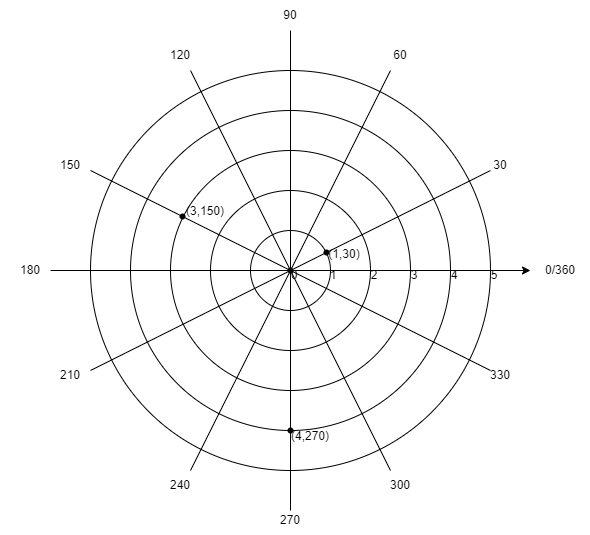
\includegraphics[scale=0.8]{polar.png}
        \end{figure}
    \end{example}

    Therefore, we shall ask a question: could we interpolate the rectangular coordinates and polar coordinates with suitable functions?

    To answer the above quesiton, we need to clarify what our desired interpolate strategy does and so we could choose a suitable set of functions to complete the interpolation.

    \subsubsection*{The interpolation}

    Let us declare the relation between rectangular plane and polar coordinates by merging them together. Observe they both have an origin (which is important to show they both have a point of respect) and thus we can stash them into one picture. We will see the following result:

    \begin{figure}[H]
        \centering
        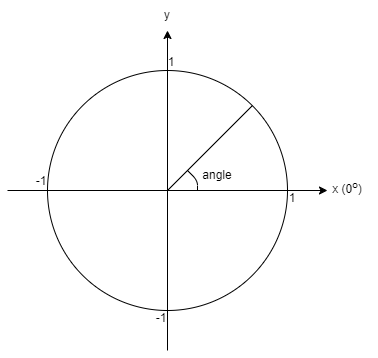
\includegraphics[scale=0.8]{rectpolar.png}
    \end{figure}

    Placing a unit circle (a circle of radius 1) on the rectangular plane, we could see that if we identify the positive x-direction as the direction of $0^\circ$ in polar coordinates, we can clearly merge two plane together. For each particular angle, we can draw a straight line to an intersection on the unit circle. Such point can be represented by a pair of rectangular coordinates, at the same time it can also be represented by a pair of polar coordinates by construction. We shall see the one-to-one correspondence between $(x,y)$ and $(r,\theta)$ if we call the angle $\theta$ and restrict its domain to $0\leq \theta < 360^\circ$. We restrict the domain to be less than $360^\circ$ because of the duplication at $0^\circ$.

    We can conclude what we need for such interpolation: some functions that relates the following pair of numbers $$(x,y)\sim (r,\theta)$$ and indeed, we can further write $$x=f_1(r,\theta), \, y=f_2(r,\theta)$$ for some functions $f_1$ and $f_2$.

    \subsubsection*{Defining trigonometry as coordinate function}

    We come to the part of configuring trigonometric functions as coordinate functions. Let us not use the notation of sine and cosine too early, since I will convince you that trigonometric functions will no longer be about triangle only with some reason behind.

    Let the discussed $f_1$ and $f_2$ be replaced by $C$ and $S$ for convenience. Then, we have to write \[x=C(r,\theta), \, y=S(r,\theta)\]

    One property of $C$ and $S$ that can easily be observed from similar triangle is that \begin{align*}
        C(r,\theta)&=rC(1,\theta)\\
        S(r,\theta)&=rS(1,\theta)
    \end{align*}
    and so we return to the unit circle for simpler observations.

    \begin{figure}[H]
        \centering
        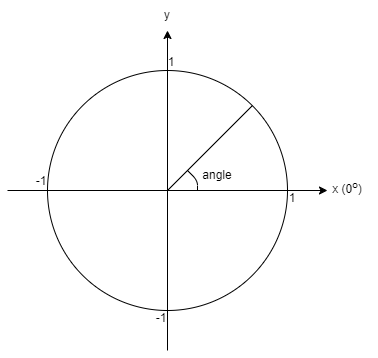
\includegraphics[scale=0.8]{rectpolar.png}
    \end{figure}

    As $C(1,\theta)$ defines the $x$-coordinate at a certain degree in a unit circle, we observe the following:\begin{itemize}
        \item When $\theta=0^\circ$, $C(1,\theta)=1$;
        \item When $\theta=90^\circ$, $C(1,\theta)=0$;
        \item When $\theta=180^\circ$, $C(1,\theta)=-1$;
        \item When $\theta=270^\circ$, $C(1,\theta)=0$.
    \end{itemize}

    In particular, if we observe for $0^\circ \leq \theta \leq 90^\circ$, the values of $C(1,\theta)$ is equivalent to seeing the length of adjeacent side of a right-angled triangle with hypotenuse 1, by definition of trigonometric functions, is exactly the value of $\cos{\theta}$. Hence, when $0^\circ\leq \theta\leq 90^\circ$, we can write $C(1,\theta)=\cos{\theta}$.

    We then say the function $C$ defined for coordinates is an extension of the standard cosine function, and we will write $\cos{\theta}$ to simplify the writings, at the same time admit the meaning of $\cos{\theta}$ when $\theta>90^\circ$ is about the $x$-coordinate on a unit circle. Hence, we will write the following $$x=r\cos{\theta}$$ for $0^\circ\leq \theta < 360^\circ$.

    Similarly, we also observe that, as $S(1,\theta)$ defines the $y$-coordinate at a certain degree in a unit circle, we have the following:\begin{itemize}
        \item When $\theta=0^\circ$, $S(1,\theta)=0$;
        \item When $\theta=90^\circ$, $S(1,\theta)=1$;
        \item When $\theta=180^\circ$, $S(1,\theta)=0$;
        \item When $\theta=270^\circ$, $S(1,\theta)=-1$.
    \end{itemize}

    In particular, if we observe for $0^\circ \leq \theta \leq 90^\circ$, the values of $S(1,\theta)$ is equivalent to seeing the length of opposite side of a right-angled triangle with hypotenuse 1, by definition of trigonometric functions, is exactly the value of $\sin{\theta}$. Hence, when $0^\circ\leq \theta\leq 90^\circ$, we can write $S(1,\theta)=\sin{\theta}$.

    We then say the function $S$ defined for coordinates is an extension of the standard sine function, and we will write $\sin{\theta}$ to simplify the writings, at the same time admit the meaning of $\sin{\theta}$ is about the $y$-coordinate on a unit circle. Hence, we will write the following $$y=r\sin{\theta}$$ for $0^\circ\leq \theta < 360^\circ$.

    Conclude the one-way implication of coordinates functions by the following relation: 

    \begin{proposition}
        Let $(r,\theta)$ be a pair of polar coordinates, with $r>0$ and $0^\circ\leq \theta<360^\circ$. We can compute the corresponding rectangular coordinates by the formula \[(x,y)=(r\cos{\theta},r\sin{\theta})\]
    \end{proposition}

    Then, how about the reverse side of implication? We shall consider the reverse side of relation \[(r,\theta)\sim (x,y)\] which can be explicitly written as \[r=g_1(x,y), \, \theta=g_2(x,y)\] for some functions $g_1$ and $g_2$.

    Let again write $g_1$ and $g_2$ into $R$ and $T$ for convenience. From the plot, it is easy to see for every pair of $x$ and $y$, we can consider the distance between the circum-point and the center of the unit circle (the origin) to be $\sqrt{(x-0)^2+(y-0)^2}=\sqrt{x^2+y^2}$. From the formula it is easy to check that $R(x,y)=\sqrt{x^2+y^2}\leq 0$ for any $(x,y)$ in the plane. We so defined \[r=R(x,y)=\sqrt{x^2+y^2}\]

    For the function $T$, it is a bit tricky. Let us consider the geometric meaning of the angle $\theta$ so that we could find a way to define the function $T$. One critical observation is the slope of the line connecting the origin and the coordinates $(x,y)$. Let the slope be $\mathfrak{M}$. Then we can write \[\mathfrak{M}=\frac{y-0}{x-0}=\frac{y}{x}\]

    Therefore, the function $T$ should be defined by another fucntion $Q$ so that $\theta=T(x,y)=Q(\frac{y}{x})$, and if there is a function $P$ such that $P\circ Q = \id$, the identity function, we can write $$P(\theta)=\frac{y}{x}$$ to observe the relation between $\theta$ and $x,y$.

    Once again, when $0^\circ \leq \theta < 90^\circ$, the value of $P(\theta)$ is exactly describing the ratio of the length of opposite side over the length of adjacent side of a right-angled triangle, which by definition is $\tan{\theta}$. Hence, we conclude when $0^\circ \leq \theta < 90^\circ$, $P(\theta)=\tan{\theta}$. As in previous deduction, we will take the extension of $\tan{\theta}$ to be describing the slope to origin on rectangular plane. Hence, we conclude the relation by taking the inverse of tangent function: \[\theta=\arctan(\frac{y}{x})\]

    Therefore, the implication from rectangular plane to polar plane, call it \textbf{polarization}, is concluded by 

    \begin{proposition}[Polarization]
        Let $(x,y)$ be a pair of rectangular coordinates. We can compute the corresponding polar coordinates by the formula \[(r,\theta)=(\sqrt{x^2+y^2},\arctan(\frac{y}{x}))\]
    \end{proposition}

    One more hint to condense the name trigonometry to describing coordinates is the consistency of trigonometric identity:

    \begin{proposition}
        Let $(x,y)\sim(r,\theta)$ be a pair of coordinate relation with discussed relating functions. The following identity holds well: \begin{enumerate}
            \item $\sin^2{\theta}+\cos^2{\theta}\equiv 1$;
            \item $\tan{\theta}\equiv\dfrac{\sin{\theta}}{\cos{\theta}}$.
        \end{enumerate}
    \end{proposition}
    
    \begin{proof}
        \begin{enumerate}
            \item Since $x=r\cos{\theta}$ and $y=r\sin{\theta}$, following the definition of $r$, \begin{align*}
                x^2+y^2&=r^2\\
                (\frac{x}{r})^2+(\frac{y}{r})^2&=1\\
                \cos^2{\theta}+\sin^2{\theta}&=1
            \end{align*}
            \item It is not hard to follow the equation deduced:\begin{align*}
                RHS&=\frac{\sin{\theta}}{\cos{\theta}}\\
                &=\frac{y/r}{x/r}\\
                &=\frac{y}{x}\\
                &=\tan{\theta}\\
                &=LHS
            \end{align*}
        \end{enumerate}
    \end{proof}

    But there's a lot more to discuss about the name `tangent' - it is not a simple discussion to explain why we call the slope of the line connecting the point and the origin by tangent function, in fact, more intuition is needed to explain that naming.

    For if any clear explanation is required, one popular saying is using the unit circle centered at origin.

    \begin{figure}[H]
        \centering
        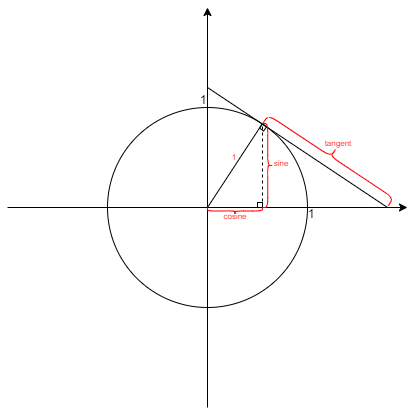
\includegraphics[scale=0.8]{trigo_on_circle.png}
    \end{figure}

    Let us revise the meaning of $\tan{\theta}$. We usually call the straight line touches the circle at point $(x,y)$ to be the \textbf{tangent line} to the circle at $(x,y)$. Note that if we would like to find the \textbf{length of tangent captured by $\theta$}, we would see the mentioned tangent as in the figure. With respect to the drawn unit circle, we could see a pair of similar triangle, which stands $$\frac{\sin{\theta}}{\cos{\theta}}=\frac{tan{\theta}}{1}$$ and such that we have the relation $\tan{\theta}=\dfrac{\sin{\theta}}{\cos{\theta}}$ same as in trigonometry. The relation accidentally computes the same result as the slope of the radius, so we take in advance the slope equals to $\tan{\theta}$.

    Using the concept of slope, we can easily describe the geometric meaning of negativity of tangent - negative slope. Therefore, this part of configuration is done.

    \subsubsection*{Reduction formula for trigonometric functions}

    According to the defined `brand new' trigonometry (coordinating functions), we may now observe the symmetric properties over those trigonometric functions. We first read the symmetry of the sine function.

    \begin{theorem}
        $\sin{(90^\circ - \theta)}=\sin{(90^\circ + \theta)}$ and $\sin{(270^\circ - \theta)}=\sin{(270^\circ + \theta)}$ for $0^\circ \leq \theta \leq 90^\circ$.
    \end{theorem}

    \begin{proof}
        For each part of the theorem, note that we may place the y-axis the common side of the triangle drawn with both radius. The congruence is trivial and hence the equality holds.
    \end{proof}

    \begin{corollary}
        $\sin{(180^\circ - \theta)}=\sin{\theta}$.
    \end{corollary}

    \begin{theorem}
        $\cos{(360^\circ - \theta)}=\cos{\theta}$ and $\cos{(180^\circ - \theta)}=\cos{(180^\circ + \theta)}$ for $0^\circ \leq \theta \leq 90^\circ$.
    \end{theorem}

    \begin{proof}
        For each part of the theorem, note that we may place the x-axis the common side of the triangle drawn with both radius. The congruence is trivial and hence the equality holds.
    \end{proof}

    With the collection from fundamental trigonometry, we have the following collection of Reduction formulae:

    \begin{theorem}
        Let $\theta$ be such that $0^\circ\leq \theta\leq 90^\circ$, the following holds: \begin{align*}
            &\sin(90^\circ\pm\theta)=\cos{\theta},&&\cos(90^\circ\pm\theta)=\mp\sin{\theta},&&\tan(90^\circ\pm\theta)=\mp\frac{1}{\tan{\theta}}\\
            &\sin(180^\circ\pm\theta)=\mp\sin{\theta},&&\cos(180^\circ\pm\theta)=-\cos{\theta},&&\tan(180^\circ\pm\theta)=\pm\tan{\theta}\\
            &\sin(270^\circ\pm\theta)=-\cos{\theta},&&\cos(270^\circ\pm\theta)=\pm\sin{\theta},&&\tan(270^\circ\pm\theta)=\mp\frac{1}{\tan{\theta}}\\
            &\sin(360^\circ - \theta)=-\sin{\theta},&&\cos(360^\circ - \theta)=\cos{\theta},&&\tan(360^\circ - \theta)=-\tan{\theta}
        \end{align*}
    \end{theorem}

    However, it was too terrifying if we need to remember all the above equalities. Is there any quick method to do with?

    \subsubsection*{The C-A-S-T graph and reduction strategy}

    Let us conclude the positivity of trigonomertric functions and see whether we can generate a useful memorization technique in order to remember the discussed reduction formulae.

    By categorizing the domain of $\theta$ into different quadrant, we could see the following picture:

    \begin{figure}[H]
        \centering
        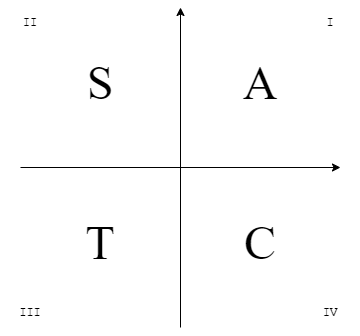
\includegraphics[scale=0.8]{C-A-S-T.png}
    \end{figure}

    From the point of view of polar coordinates, we count for the first 90 degree as quadrant I; the second 90 degree as quadrant II; the third 90 degree as quadrant III; the fourth 90 degree as quadrant IV. 

    The discussion on different quadrant provides different sign of axis. We concludes the following.

    Quadrant I is where both $x$ and $y$ coordinates being positive, and we can observe that for every trigonometric function in quadrant I, they are all positive. That is, for $0^\circ<\theta<90^\circ$, \begin{align*}
        \sin{\theta} &> 0\\
        \cos{\theta} &> 0\\
        \tan{\theta} &> 0
    \end{align*}
    Hence, the results show that ALL trigonometric functions are positive, and we name quadrant I by `A' to amplify the phenomenon.

    Quadrant II is where only $y$ coordinates being positive, and we can observe that for trigonometric functions in quadrant I, only sine function is positive. That is, for $90^\circ<\theta<180^\circ$, \begin{align*}
        \sin{\theta} &> 0\\
        \cos{\theta} &< 0\\
        \tan{\theta} &< 0
    \end{align*}
    Hence, the results show that only Sine is positive, and we name quadrant II by `S' to amplify the phenomenon.

    Quadrant III is where no coordinate is positive, and we can observe that for trigonometric functions in quadrant III, only tangent function is positive. That is, for $180^\circ<\theta<270^\circ$, \begin{align*}
        \sin{\theta} &< 0\\
        \cos{\theta} &< 0\\
        \tan{\theta} &> 0
    \end{align*}
    Hence, the results show that only Tangent is positive, and we name quadrant III by `T' to amplify the phenomenon.

    Quadrant IV is where only $x$ coordinates being positive, and we can observe that for trigonometric functions in quadrant IV, only cosine function is positive. That is, for $270^\circ<\theta<360^\circ$, \begin{align*}
        \sin{\theta} &< 0\\
        \cos{\theta} &> 0\\
        \tan{\theta} &< 0
    \end{align*}
    Hence, the results show that only Cosine is positive, and we name quadrant IV by `C' to amplify the phenomenon.

    What's special about this naming technique is that we can memorize the quadrants of positivity by spelling C-A-S-T, the CAST graph, to simply guess the required sign of reduction.

    Another important observation to fast-guess the reduction formula is paying attention to previous theorem, which, said \begin{align*}
        &\sin(180^\circ\pm\theta)=\mp\sin{\theta},&&\cos(180^\circ\pm\theta)=-\cos{\theta},&&\tan(180^\circ\pm\theta)=\pm\tan{\theta}\\
        &\sin(360^\circ - \theta)=-\sin{\theta},&&\cos(360^\circ - \theta)=\cos{\theta},&&\tan(360^\circ - \theta)=-\tan{\theta}
    \end{align*}

    It is important to notice that we don't need to change the functions into another functions when the leading angle is $180^\circ$ or $360^\circ$. On the other hand, the not a multiple of 180, the conversion behave like \[\sin \mapsto \cos, \cos \mapsto \sin, \tan \mapsto \frac{1}{\tan}\]

    Therefore, the strategy of reduction can be summarized by following: \begin{enumerate}
        \item Sign-deduction: by CAST;
        \item Function-deduction: by multiple of $180^\circ$.
    \end{enumerate}

    \subsection{Extending trigonometry to any degree}

    We known from definition of polar coordinates that we can reduce angle over $360^\circ$ to less than it. The rotation deforms by subtracting or adding whole circles to the angle according to its positivity and magnitudes. We therefore access to any degree with trigonometric functions.

    \subsubsection*{periodic function}

    Taking advantages from polar plane, we can write down an equivalence class of angle: \[360^\circ + \theta \equiv \theta\] and so we can write the following extension of angle formulae:\begin{align*}
        \sin{(360^\circ + \theta)}&=\sin{\theta}\\
        \cos{(360^\circ + \theta)}&=\cos{\theta}\\
        \tan{(360^\circ + \theta)}&=\tan{\theta}
    \end{align*}

    For the above situation, we name the $360^\circ$ as the \textbf{period} of polar coordinates, and also the period of trigonometric functions $\sin, \cos$ and $\tan$. Alternatively, we say those trigonometric functions are \textbf{periodic functions} with period $360^\circ$, with following definition of periodic functions.
    
    \begin{definition}[periodic function]
        Let $T$ be a number and $f$ be a function. If for any real number $x$, the function $f$ always satisfy the equation \[f(x+T)=f(x)\] then we call $f$ a periodic function with period $T$.
    \end{definition}

    To visualize the periodicity of trigonometric functions, we plot the graphs out.

    \begin{example}
        Graph of sine function:

        \begin{center}
            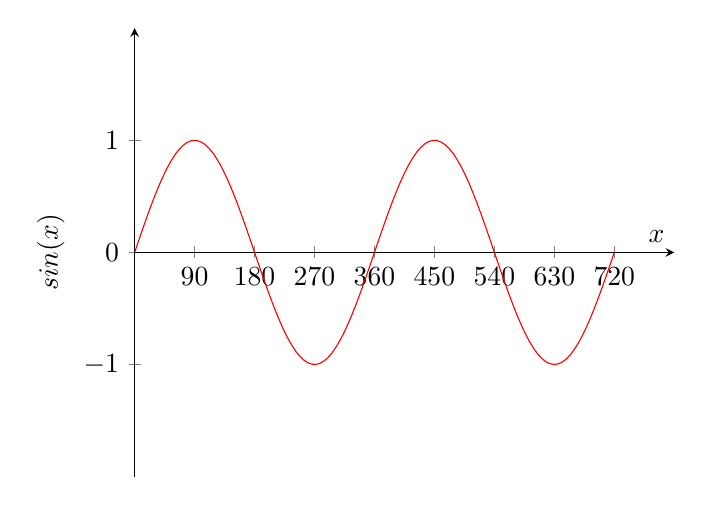
\begin{tikzpicture}
                \begin{axis}[
                axis y line = left,
                axis x line = middle,
                xlabel = \(x\),
                ylabel = {\(sin(x)\)},
                xmin=0, xmax=810,
                ymin=-2, ymax=2,
                xtick={90,180,270,360,450,540,630,720},
                ytick={-1,0,1}
                ]
                \addplot [
                    domain=0:720, 
                    samples=120, 
                    color=red,
                ]
                {sin(x)};
                \end{axis}
            \end{tikzpicture}            
        \end{center}

        We shall observe that the sine function starts at 0, maximized and minimized at $1$ and $-1$ respectively. The value of $\sin{x}$ at $x=0^\circ$ is equal to at $x=360^\circ$, that at $x=90^\circ$ is equal to at $x=450^\circ$, etc. It looks like a copt-and-paste action to draw the curve after $360^\circ$.
    \end{example}

    \begin{example}
        Graph of cosine function:

        \begin{center}
            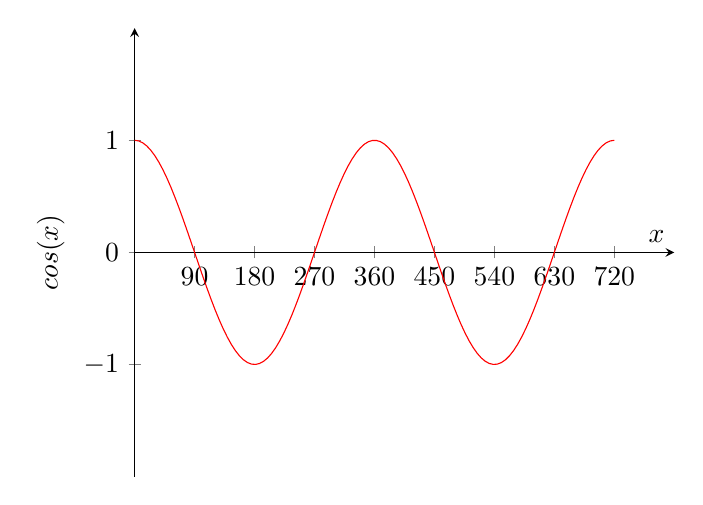
\begin{tikzpicture}
                \begin{axis}[
                axis y line = left,
                axis x line = middle,
                xlabel = \(x\),
                ylabel = {\(cos(x)\)},
                xmin=0, xmax=810,
                ymin=-2, ymax=2,
                xtick={90,180,270,360,450,540,630,720},
                ytick={-1,0,1}
                ]
                \addplot [
                    domain=0:720, 
                    samples=120, 
                    color=red,
                ]
                {cos(x)};
                \end{axis}
            \end{tikzpicture}            
        \end{center}

        We shall observe that the cosine function starts at 1, maximized and minimized at $1$ and $-1$ respectively. The value of $\cos{x}$ at $x=0^\circ$ is equal to at $x=360^\circ$, that at $x=90^\circ$ is equal to at $x=450^\circ$, etc. It looks like a copt-and-paste action to draw the curve after $360^\circ$.
    \end{example}

    \begin{example}
        Graph of tangent function:

        \begin{center}
            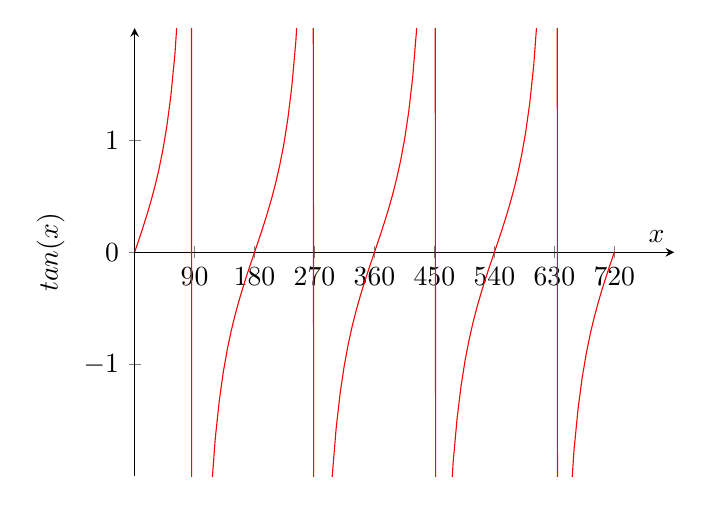
\begin{tikzpicture}
                \begin{axis}[
                axis y line = left,
                axis x line = middle,
                xlabel = \(x\),
                ylabel = {\(tan(x)\)},
                xmin=0, xmax=810,
                ymin=-2, ymax=2,
                xtick={90,180,270,360,450,540,630,720},
                ytick={-1,0,1}
                ]
                \addplot [
                    domain=0:720, 
                    samples=120, 
                    color=red,
                ]
                {tan(x)};
                \end{axis}
            \end{tikzpicture}            
        \end{center}

        We shall observe that the tangent function starts at 0, increasing all the time. It has no maxima or minima, however, still periodic. The value of $\tan{x}$ at $x=0^\circ$ is equal to at $x=360^\circ$, that at $x=90^\circ$ is equal to at $x=450^\circ$, etc. It looks like a copt-and-paste action to draw the curve after $360^\circ$.
    \end{example}

    \subsubsection*{Extending domain and bounded range}

    \subsection{Challenging Questions}

    \newpage

    \section{Linear functions}

    In this section, we focus on a specific form of function, which is called \textbf{Linear functions}, a type of functions that generate straight lines in the Euclidean space, or we may call it the xy-plane, denoted by $\mathbb{R}^2$. It is the simplest form of function, and has many properties we are interested in.

    \subsection{Fundamental concepts of points}

    Revisiting the xy-plane, we may define some useful tools for measurement and ratio properties, since we shall always be equipped with the sense of measuring and performing comparisons.

    \subsubsection*{Distance between two points}

    One important practical measurement in the xy-plane is the so-called \textbf{distance between two points}. We recall that given a right-angled triangle $\triangle ABC$ with $\angle ABC = 90^\circ$, the following relation on the side lengths holds: $$|\overline{AB}|^2+|\overline{BC}|^2=|\overline{AC}|^2$$ where the stroke sign $|\cdot|$ denotes the length of a certain line and each line is mentioned explicitly using the over-lined notation $\overline{XY}$ to indicate the line connecting point $X$ and point $Y$. As we learned the relation is mentioned by \textit{Pythagoras Theorem} or \textit{Pythagorean Theorem}.
    
    Following from the Pythagoras Theorem, we shall examine the distance between any two points on the xy-plane by the length of the straight line connecting them. With the help of the following figure, let us carry out our definition of distance between two points.

    \begin{definition}[Distance between two points]
        Let $A(x_1,y_1)$ and $B(x_2,y_2)$ be two points on $\mathbb{R}^2$-plane. The distance between $A$ and $B$ is computed by the formula $$\mathrm{dist}(A,B):=\sqrt{(x_1-x_2)^2+(y_1-y_2)^2}$$
    \end{definition}

    We may think of the following construction for distance between two points:

    Taking the right-angled triangle as distance reference, the vertical displacement becomes $|y_1-y_2|$ and the horizontal displacement becomes $|x_1-x_2|$. Putting the oblique displacement $\mathrm{dist}(A,B)$ gives the Pythagorean relation, and we could get the desired formula.

    \begin{example}
        Let $A(1,2)$ and $B(4,-2)$ be two points on the rectangular coordinate plane, i.e. the xy-plane. Then, $$\mathrm{dist}(A,B)=\sqrt{(1-4)^2+(2-(-2))^2}=\sqrt{3^2+4^2}=\sqrt{25}=5$$
    \end{example}

    \begin{example}
        Let $A(1,2)$ and $B(k,k-1)$ be two points on the rectangular coordinate plane such that $\mathrm{dist}(A,B)=2$. Then, \begin{align*}
            \sqrt{(k-1)^2+(k-3)^2}&=2\\
            (k-1)^2+(k-3)^2&=4\\
            k^2-2k+1+k^2-6k+9&=4\\
            2k^2-8k+6&=0\\
            k^2-4k+3&=0\\
            (k-1)(k-3)&=0\\
        \end{align*}
        Then $k=1$ or $k=3$, i.e. the possible coordinates of $B$ are $(1,0)$ or $(3,2)$.
    \end{example}

    \begin{example}
        Given two trajectories $T_1:(x_1(t),y_1(t))$ and $T_2:(x_2(t),y_2(t))$, we say the distance between $T_1$ and $T_2$ is $$\mathrm{dist}(T_1,T_2):=\min_{t>0}\sqrt{(x_1(t)-x_2(t))^2+(y_1(t)-y_2(t))^2}$$
    \end{example}

    It is quite abstract to talk about the distance between two trajectories in this stage. Just keep in mind that this is a truth, or say you may believe in it.

    \begin{exercise}
        Compute the distance between following pair of points:\begin{enumerate}
            \item $(1,0)$ and $(0,1)$;
            \item $(1,-1)$ and $(-1,1)$;
            \item $(3,4)$ and $(12,-13)$;
            \item $(7,-8)$ and $(-3,0)$;
        \end{enumerate}
    \end{exercise}

    \begin{exercise}
        Given the distance between two points, find the possible value(s) of the unknowns:\begin{enumerate}
            \item $A(0,0), B(3,k)$; $\mathrm{dist}(A,B)=3$.
            \item $A(2,0), B(3,k)$; $\mathrm{dist}(A,B)=1$.
            \item $A(k,0), B(0,k)$; $\mathrm{dist}(A,B)=5$.
            \item $A(3+k,1-k), B(3,-3)$; $\mathrm{dist}(A,B)=8$.
        \end{enumerate}
    \end{exercise}

    \subsubsection*{Mid-point and Division points}

    \begin{definition}[Mid-way of a trajectory]
        Given a trajectory defined by $(x(t),y(t))$ where $t\in [0,r]$ with $r>0$ a real number, the \textbf{midway} (or \textbf{half-way}) of the trajectory is given by the point $M$ such that $$\mathrm{arclength}((x(0),y(0)),M)=\mathrm{arclength}(M,(x(r),y(r)))$$
    \end{definition}

    In particular, if we are talking about a mid-point, we usually pick the shortest trajectory between the two points. This is due to the uniqueness of the shortest trajectory if our distance is well-defined. In the Euclidean space, the shortest trajectory is usually the straight line between the two points.

    \begin{theorem}[Mid-point of two points]
        Given $A(x_1,y_1)$ and $B(x_2,y_2)$ be two points on the Euclidean space, the \textbf{mid-point} $M$ of $A$ and $B$ is defined by $$(\frac{x_1+x_2}{2},\frac{y_1+y_2}{2})$$
    \end{theorem}

    \begin{proof}
        Let $L$ be the straight line connecting $A$ and $B$. Assume that $M:=(\dfrac{x_1+x_2}{2},\dfrac{y_1+y_2}{2})$, then\begin{align*}
            \mathrm{dist}(A,M)&=\sqrt{(x_1-\frac{x_1+x_2}{2})^2+(y_1-\frac{y_1+y_2}{2})^2}\\
            &=\frac{1}{2}\sqrt{(x_1-x_2)^2+(y_1-y_2)^2}\\
            &=\frac{1}{2}\mathrm{dist}(A,B)\\
            \mathrm{dist}(M,B)&=\sqrt{(\frac{x_1+x_2}{2}-x_2)^2+(\frac{y_1+y_2}{2}-x_2)^2}\\
            &=\frac{1}{2}\sqrt{(x_1-x_2)^2+(y_1-y_2)^2}\\
            &=\frac{1}{2}\mathrm{dist}(A,B)\\
        \end{align*}
        In particular, $$\mathrm{dist}(A,M)+\mathrm{dist}(M,B)=\mathrm{dist}(A,B)$$
        Thus $M$ preserve a point on the straight line connecting $A$ and $B$ and in fact the mid-point of $A$ and $B$.
    \end{proof}

    \begin{example}
        Given $A(100,20)$ and $B(30,70)$, their mid-point is the point $M(65,45)$.
    \end{example}

    \begin{exercise}
        For the following given pairs of points, find their mid-points:\begin{enumerate}
            \item $(2,2)$ and $(0,0)$;
            \item $(2,1)$ and $(-2,-1)$.
        \end{enumerate}
    \end{exercise}

    Other than the mid-point, we also consider the general version of line separation, which is the point of division.

    \begin{definition}[Point of division]
        Given two points $A$ and $B$, any point $P$ lies in between $A$ and $B$ is called \textbf{the point of division with ratio $\mathrm{dist}(A,P):\mathrm{dist}(P,B)$}.
    \end{definition}

    \begin{theorem}[Formula for point of division]
        Let $A(x_1,y_1)$ and $B(x_2,y_2)$ be a point on the Euclidean space. Let $P$ be the point of division of $A$ and $B$ with ratio $r:s$. Then the coordinates of $P$ is given by $$\frac{sA+rB}{r+s}=(\frac{sx_1+rx_2}{r+s},\frac{sy_1+ry_2}{r+s})$$ In particular, the mid-point of $A$ and $B$ is given by setting $s=r=1$.
    \end{theorem}

    \begin{proof}
        Similar to the proof of mid-point. Let $P:=(\dfrac{sx_1+rx_2}{r+s},\dfrac{sy_1+ry_2}{r+s})$, then\begin{align*}
            \mathrm{dist}(A,P)&=\sqrt{(x_1-\frac{sx_1+rx_2}{r+s})^2+(y_1-\frac{sy_1+ry_2}{r+s})^2}\\
            &=\frac{1}{r+s}\sqrt{(rx_1-rx_2)^2+(ry_1-ry_2)^2}\\
            &=\frac{r}{r+s}\mathrm{dist}(A,B)\\
            \mathrm{dist}(P,B)&=\sqrt{(\frac{sx_1+rx_2}{r+s}-x_2)^2+(\frac{sy_1+ry_2}{r+s}-x_2)^2}\\
            &=\frac{1}{r+s}\sqrt{(sx_1-sx_2)^2+(sy_1-sy_2)^2}\\
            &=\frac{s}{r+s}\mathrm{dist}(A,B)\\
        \end{align*}
        In particular, $$\mathrm{dist}(A,P)+\mathrm{dist}(P,B)=\mathrm{dist}(A,B)$$
        Thus $P$ preserve a point on the straight line connecting $A$ and $B$ and satisfies $\mathrm{dist}(A,P):\mathrm{dist}(P,B)=\dfrac{r}{r+s}:\dfrac{s}{r+s}=r:s$.
    \end{proof}

    \begin{example}
        Let $A(2,4)$ and $B(-4,7)$. To trisect the line connecting $A$ and $B$, we need two points on the line where they divide the straight line in the ratio of $1:1:1$. In particular, let the point closer to $A$ be $X$ and the other be $Y$, we have $X$ the division point of ratio $1:2$ and $Y$ the division point of ratio $2:1$. Therefore,\begin{align*}
            X:&=(\frac{2(2)+1(-4)}{1+2}, \frac{2(4)+1(7)}{1+2})=(0,5)\\
            Y:&=(\frac{1(2)+2(-4)}{1+2}, \frac{1(4)+2(7)}{1+2})=(-2,6)\\
        \end{align*}
    \end{example}

    \begin{exercise}
        Given $A(-100,-10)$ and $B(100,100)$. Find the point of division for the following given ratio $r:s$ :\begin{enumerate}
            \item $r:s=1:1$;
            \item $r:s=1:3$;
            \item $r:s=3:7$;
            \item $r:s=19:91$.
        \end{enumerate}
    \end{exercise}

    \subsubsection*{Slope of two points}

    For two points, we want to know not only how far away they are, but also how steep they see each other, i.e. the direction of proceeding. We call it the slope of the two points.

    To be professional, we say a slope of the two points is how line goes from the left point to the right point; that is, whether $y$ increase with $x$ or $y$ decrease with $x$.

    \begin{definition}[Slope]
        Let $A(x_1,y_1)$ and $B(x_2,y_2)$ be two points on the Euclidean space. Then the \textbf{slope} of $A$ and $B$, denoted by $\mathfrak{M}_{AB}$, is given by $$\mathfrak{M}_{AB}:=\frac{y_2-y_1}{x_2-x_1}$$
    \end{definition}

    \begin{example}
        The slope of $A(1,2)$ and $B(4,1)$ is $\mathfrak{M}_{AB}=\dfrac{1-2}{4-1}=-\dfrac{1}{3}$.
    \end{example}

    We could observe the following fact. For if two points are aligned horizontally on the plane, then their slope is computed equal to 0; if the right point is higher than the left, then the slope is positive, meaning the corresponding line is increasing with $x$; otherwise the slope is negative, meaning the corresponding line is decreasing with $x$. For if two points are aligned vertically on the plane, then the slope is undefined, since we could not explicitly tell whether the corresponding line is increasing or decreasing - it could be both. Due to the uncertainty, we identify it as undefined slope. However, we can still define the slope of vertical lines for consistent usage, but that's another page of discussion.

    \begin{exercise}
        Compute the slope of the following pairs of points:\begin{enumerate}
            \item $(1,0)$ and $(0,1)$;
            \item $(1,-1)$ and $(-1,1)$;
            \item $(3,4)$ and $(12,-13)$;
            \item $(7,-8)$ and $(-3,0)$;
        \end{enumerate}
    \end{exercise}

    \begin{definition}[Collinear]
        3 points are called \textbf{collinear} if there is a straight line passes through 3 points at the same time.
    \end{definition}

    In fact, collinearity is somehow the converse of computing points of division, by the definition of point of division. We will make use of the equivalence in proving the following theorem:

    \begin{theorem}
        3 points on the plane are collinear if and only if the slope of any two of the three points are the same.
    \end{theorem}

    \begin{proof}
        For the direction from collinear to slope equality, we have if 3 points are collinear, then they can be written as $$A(x_1,x_2), B(\frac{sx_1+rx_2}{r+s}, \frac{sy_1+ry_2}{r+s}), C(x_2,y_2)$$
        We then have \begin{align*}
            \mathfrak{M}_{AB}&=\frac{\frac{sy_1+ry_2}{r+s}-y_1}{\frac{sx_1+rx_2}{r+s}-x_1}\\
            &=\frac{sy_1+ry_2-(r+s)y_1}{sx_1+rx_2-(r+s)x_1}\\
            &=\frac{ry_2-ry_1}{rx_2-rx_1}\\
            &=\frac{y_2-y_1}{x_2-x_1}\\
            \mathfrak{M}_{BC}&=\frac{y_2-\frac{sy_1+ry_2}{r+s}}{x_2-\frac{sx_1+rx_2}{r+s}}\\
            &=\frac{(r+s)y_2-sy_1+ry_2}{(r+s)x_2-sx_1+rx_2}\\
            &=\frac{sy_2-sy_1}{sx_2-sx_1}\\
            &=\frac{y_2-y_1}{x_2-x_1}\\
            \mathfrak{M}_{AC}&=\frac{y_2-y_1}{x_2-x_1}
        \end{align*}
        Then collinear implies the equality of the slopes.

        Conversely, suppose 3 points $A,B,C$ such that $\mathfrak{M}_{AB}=\mathfrak{M}_{BC}=\mathfrak{M}_{AC}=m$. We may compute that \begin{align*}
            \mathrm{dist}(A,B)&=\sqrt{(x_A-x_B)^2+(y_A-y_B)^2}\\
            &=|x_A-x_B|\sqrt{1+\mathfrak{M}_{AB}^2}
        \end{align*}
        Similarly, we have \begin{align*}
            \mathrm{dist}(B,C)&=|x_B-x_C|\sqrt{1+\mathfrak{M}_{BC}^2}\\
            \mathrm{dist}(A,C)&=|x_A-x_C|\sqrt{1+\mathfrak{M}_{AC}^2}
        \end{align*}
        Without loss of generality, we may assume their x-coordinates are in fixed order, where I will set $x_A<x_B<x_C$. Then \begin{align*}
            \mathrm{dist}(A,B)+\mathrm{dist}(B,C)&=(|x_A-x_B|+|x_B-x_C|)\sqrt{1+m^2}\\
            &=(x_B-x_A+x_C-x_B)\sqrt{1+m^2}\\
            &=|x_A-x_C|\sqrt{1+\mathfrak{M}_{AC}^2}\\
            &=\mathrm{dist}(A,C)
        \end{align*}
        This shows that $B$ is a point of division of $A$ and $C$, and hence $A,B,C$ are collinear.
    \end{proof}

    \begin{corollary}
        3 points on the plane are not collinear if and only if the slope of any two of the three points are not the same.
    \end{corollary}

    By the theorem, we could easily show the collinearity of any 3 points, and of course we may push a little forward from it.
    
    \begin{example}
        Determine the collinearity of following sets of points:\begin{enumerate}
            \item $(0,0), (1,2), (2,4)$.\\
            \textit{ Sol. } Denote $(0,0), (1,2), (2,4)$ by $A,B,C$ respectively. Then \begin{align*}
                \mathfrak{M}_{AB}&=\frac{2-0}{1-0}=2\\
                \mathfrak{M}_{BC}&=\frac{4-2}{2-1}=2
            \end{align*}
            Then, by the previous theorem, $A,B,C$ are collinear.
            \item $(0,1), (1,2), (2,2)$.\\
            \textit{ Sol. } Denote $(0,0), (1,2), (2,4)$ by $A,B,C$ respectively. Then \begin{align*}
                \mathfrak{M}_{AB}&=\frac{2-1}{1-0}=2\\
                \mathfrak{M}_{BC}&=\frac{2-2}{2-1}=0
            \end{align*}
            Then, by the previous theorem, $A,B,C$ are not collinear.
        \end{enumerate}
    \end{example}

    \begin{exercise}
        Determine the collinearity of the following sets of points:\begin{enumerate}
            \item $(0,0), (1,3), (2,6)$.
            \item $(1,0), (0,-1), (-1,-2)$.
            \item $(0,2), (1,-3), (-2,6)$.
            \item $(k,4), (4+k,4+k), (4,k)$.
        \end{enumerate}
    \end{exercise}

    This measurement provides another way of line construction. In fact, by one of its powerful property, there is a generalized version of slope with various application in higher mathematics and other fields including computer science.

    \begin{theorem}[Invariant properties of slope of two points]
        Let $A$ and $B$ be two points on the Euclidean space, and $\mathfrak{M}_{AB}$ be the slope of $A$ and $B$. Under any simultaneous translation to $A$ and $B$, $\mathfrak{M}_{AB}$ remains unchanged.
    \end{theorem}

    \begin{proof}
        Let $A(x_1,y_1)$ and $B(x_2,y_2)$ be two points. Suppose $A'$ and $B'$ be the resulting coordinates after simultaneously translating $A$ and $B$, we may write $A'(x_1+\Delta x, y_1+\Delta y)$ and $B'(x_2+\Delta x, y_2+\Delta y)$. Then the slope after simultaneous translation is $$\mathfrak{M}_{A'B'}=\frac{(y_2+\Delta y)-(y_1+\Delta y)}{(x_2+\Delta x)-(x_1+\Delta x)}=\frac{y_2-y_1}{x_2-x_1}=\mathfrak{M}_{AB}$$
    \end{proof}

    \subsection{Different forms of a linear function}

    Following the concepts of distance, point of division and slope, we can now discuss the form of a linear function.

    \subsubsection*{Segment}

    We may first consider a segment in the plane, which is the straight line connecting any two points in the Euclidean plane, ends at that two points.

    \begin{definition}[Segment]
        A \textbf{segment} with two endpoints $A$ and $B$ is the collection of all division points between $A$ and $B$. In other words, it is a straight line with endpoints $A$ and $B$.
    \end{definition}

    By the definition of division point, we may let $A(x_1,y_1)$ and $B(x_2,y_2)$ be two points, and two numbers $r$ and $s$ such that every division point of ratio $r:s$ could be represented in the following form $$(\frac{sx_1+rx_2}{r+s},\frac{sy_1+ry_2}{r+s})$$

    By simple algebra, we can see that $\dfrac{s}{r+s}=1-\dfrac{r}{r+s}$, so we may let $t:=\dfrac{r}{r+s}$ be a number in between 0 and 1 such that every division point can be written as $$((1-t)x_1+tx_2, (1-t)y_1+ty_2)=(x_1+t(x_2-x_1),y_1+t(y_2-y_1))$$ with $0\leq t\leq 1$. Now, we could see the relationship between x- and y- coordinates in the following derivation:\begin{align*}
        y:&=(1-t)y_1+ty_2\\
        &=y_1+t(y_2-y_1)\\
        &=y_1+t\frac{y_2-y_1}{x_2-x_1}(x_2-x_1)\\
        &=y_1+t\mathfrak{M}_{AB}(x_2-x_1)\\
        &=y_1+\mathfrak{M}_{AB}(x-x_1)
    \end{align*}

    \subsubsection*{Line as extension of a segment}

    We have established that a segment can be represented by the equation $$y=y_1+\mathfrak{M}_{AB}(x-x_1)$$
    where it is interesting to see the equation involves no variable $t$. In fact, it is independent of $t$ and could be extended to out of the segment. We call this extension a \textbf{straight line} passes through $A$ and $B$.

    The above equation looks simple, but let us confirm that the derived equation is indeed satisfying the extension of a segment. We shall return to the fundamental form of a segment but revising the domain of $t$: $$((1-t)x_1+tx_2, (1-t)y_1+ty_2)$$ where $-\infty<t<\infty$. In fact, a line should be proven to be this form rigorously. Let us dive into it.

    \begin{theorem}
        A straight line passes through $(x_1,y_1)$ and $(x_2, y_2)$ is in the form of $$((1-t)x_1+tx_2, (1-t)y_1+ty_2)$$ where $-\infty<t<\infty$.
    \end{theorem}

    \begin{proof}
        The major discussion is the domain of $t$ diverges to infinity. Let us prove first that for every real value $t$, the point $((1-t)x_1+tx_2, (1-t)y_1+ty_2)$ is collinear with $A(x_1,y_1)$ and $B(x_2,y_2)$. In fact, $$\mathfrak{M}=\frac{(1-t)y_1+ty_2-y_1}{(1-t)x_1+tx_2-x_1}=\frac{y_2-y_1}{x_2-x_1}$$ is true for all $t\neq 0$. At the same time, the case $t=0$ is just considering $(x_1,y_1)$, which is immediately true. Hence, every point in that form is collinear with $A$ and $B$.

        Next, we shall show that $t$ diverges at both ends. Suppose on contrary that $t$ is bounded above by $M$, then the longest segment ends at $V_M((1-M)x_1+Mx_2, (1-M)y_1+My_2)$, but letting $V_{M+1}((-M)x_1+(M+1)x_2, (-M)y_1+(M+1)y_2)$\begin{align*}
            \mathrm{dist}(A,V_{M+1})=(M+1)\mathrm{dist}(A,B)>M\mathrm{dist}(A,B)=\mathrm{dist}(A,V_M)
        \end{align*}
        This contradicts that $AV_M$ is the longest segment we have. Thus $t$ is unbounded. The argument is similar for $t$'s lower bound and hence $-\infty<t<\infty$.
    \end{proof}

    \subsubsection*{Point-slope form}

    Observe that $$y=y_1+\mathfrak{M}_{AB}(x-x_1) \iff y-y_1=\mathfrak{M}_{AB}(x-x_1) \iff \frac{y-y_1}{x-x_1}=\mathfrak{M}_{AB}$$ for given points $A(x_1,y_1)$ and slope $\mathfrak{M}_{AB}$, we may give the following result.

    \begin{theorem}
        If a line $L$ passes through point $A(x_1,y_1)$ and having slope $\mathfrak{M}$, then $L$ can be constructed from writing $$L:\frac{y-y_1}{x-x_1}=\mathfrak{M}$$
    \end{theorem}

    The meaning of this form can be thought of as: Given any point $(x,y)$ on the line $L$, its slope with $A$ is the same as the given slope $\mathfrak{M}$.

    \begin{example}
        Suppose $L$ is a straight line passes through $(0,0)$ with slope being equal to $3$. Then $L$ could be modified as $$L:\frac{y-0}{x-0}=3\iff y=3x$$
    \end{example}
    
    \begin{example}
        Suppose $L$ is a straight line passes through $(1,2)$ with slope being equal to $4$. Then $L$ could be modified as $$L:\frac{y-2}{x-1}=4\iff y=4x-2$$
    \end{example}

    \subsubsection*{Two-point form}

    With any two given points on the Euclidean plane, we could rewrite the slope $\mathfrak{M}$ into $\dfrac{y_2-y_1}{x_2-x_1}$. This means the line passes through any two given points could be modelled by 

    \begin{theorem}
        If a line $L$ passes through point $A(x_1,y_1)$ and $B(x_2,y_2)$, then $L$ can be constructed from writing $$L:\frac{y-y_1}{x-x_1}=\frac{y_2-y_1}{x_2-x_1}$$
    \end{theorem}

    \begin{example}
        Suppose $L$ is a straight line passes through $(0,0)$ and $(1,2)$. Then $L$ could be modified as $$L:\frac{y-0}{x-0}=\frac{2-0}{1-0}\iff y=2x$$
    \end{example}
    
    \begin{example}
        Suppose $L$ is a straight line passes through $(1,2)$ and $(10,3)$. Then $L$ could be modified as $$L:\frac{y-2}{x-1}=\frac{3-1}{10-2}\iff y=\frac{1}{4}x+\frac{7}{4}$$
    \end{example}

    \subsubsection*{Slope-intercept form}

    Given the slope $\mathfrak{M}$ and the y-intercept $c$, we could take the y-intercept as one particular coordinate $(0,c)$. This means the line with given information is 

    \begin{theorem}
        If a line $L$ has slope $\mathfrak{M}$ and y-intercept $c$, then $L$ can be constructed from writing $$L:\frac{y-c}{x-0}=\mathfrak{M}$$
    \end{theorem}

    \begin{example}
        Suppose $L$ is a straight line with slope $5$ and y-intercept $0$. Then $L$ could be modified as $$L:\frac{y-0}{x-0}=5\iff y=5x$$
    \end{example}
    
    \begin{example}
        Suppose $L$ is a straight line with slope $\frac{1}{10}$ and y-intercept $5$. Then $L$ could be modified as $$L:\frac{y-5}{x-0}=\frac{1}{10}\iff y=\frac{1}{10}x+5$$
    \end{example}

    \subsubsection*{Intercepts form}

    Except the previous forms, an intercepts form is a form purely taken from the two intercepts. Let $a$ be the x-intercept and $b$ be the y-intercept of a line $L$. We see from the view of division point, the line shall be formed by writing $$((1-t)a, tb)$$ for all the points on $L$, where $-\infty<t<\infty$. We could derive that $$\frac{x}{a}+\frac{y}{b}=1$$ for any value of $t$.

    \begin{theorem}
        Let $L$ be having x-intercept $a$ and y-intercept $b$. Then $L$ could be modelled by $$L:\frac{x}{a}+\frac{y}{b}=1$$
    \end{theorem}

    \begin{example}
        Suppose $L$ has x-intercept $5$ and y-intercept $5$. Then $L$ could be modified as $$L:\frac{x}{5}+\frac{y}{5}=1\iff y=5-x$$
    \end{example}
    
    \begin{example}
        Suppose $L$ is a straight line with x-intercept $k$ and no y-intercept. Then $L$ could be modified as $$L:\frac{x}{k}=1\iff x=k$$
    \end{example}
    
    \begin{example}
        Suppose $L$ is a straight line with y-intercept $k$ and no x-intercept. Then $L$ could be modified as $$L:\frac{y}{k}=1\iff y=k$$
    \end{example}
    
    \begin{example}
        Suppose $L$ is a straight line completely lies on x-axis. This means x-intercept is undefined. Then $L$ could be modified as $$L:y=0$$
    \end{example}
    
    \begin{example}
        Suppose $L$ is a straight line completely lies on y-axis. This means y-intercept is undefined. Then $L$ could be modified as $$L:x=0$$
    \end{example}

    \subsubsection*{General form}

    In convenience to solving linear equations, we aim to set a form that is always constructive. We put our attention to what a general form is.

    Recall that a straight line could be either a vertical line, an oblique line, or a horizontal line. We shall introduce a form that is generally true to write a straight line. This thought should eliminate the presence of slope. Perhaps the intercepts form provides a good start to write a general form. Indeed, $$\frac{x}{a}+\frac{y}{b}=1 \iff bx+ay=ab$$ gives us the form purely by multiplication and addition. This can so be rearranged such that $$bx+ay=ab\iff Ax+By+C=0$$ with $A=b$, $B=a$ and $C=-ab$. Of its elimination of slope, this is the desired form of a straight line.

    \begin{theorem}
        Any straight line $L$ can be written in the form of $$Ax+By+C=0$$ where $A,B,C$ are constants. Furthermore, the slope of $L$ is determined $-\frac{A}{B}$, the x-intercept $-\frac{C}{A}$ and y-intercept $-\frac{C}{B}$.
    \end{theorem}

    \begin{proof}
        The first part of the proof is to determine the connection between different forms of equation of straight line. Indeed, the point-slope form connects with two-point form, while the point-slope form also connects with slope intercept form. The general form comes form intercepts form, so it remains to show the connection between slope intercept form and general form. In fact, \begin{align*}
            y=\mathfrak{M}x+c &\iff \mathfrak{M}x-y+c=0\\
            &\iff Ax+By+C=0
        \end{align*}
        shows the connection between slope-intercept form and general form. This completes the first part.

        The second part of the proof should show the "furthermore" implication. Consider the definitions of x-intercept and y-intercept, we will see if $x_0$ denotes the x-intercept, then $Ax_0+B(0)+C=0$ implies $x_0=-\frac{C}{A}$; Similarly, denoting $y_0$ the y-intercept, we have $y_0=-\frac{C}{B}$. For the slope we take the provided intercepts and write $$\mathfrak{M}=\frac{y_0-0}{0-x_0}=-\frac{A}{B}$$ concludes the proof.
    \end{proof}

    It is the best to write the general form with integers instead of fractions or decimal numbers, since it is more convenient and intuitive to solve equations using integers. In general, if we have to handle irrational numbers, we prefer to write everything without quotient and shall be simplest.

    \begin{example}
        It is better to write $x+2y+3=0$ instead of $\frac{1}{2}x+y+\frac{3}{2}=0$.
    \end{example}

    \begin{example}
        If we need to handle irrationals, say $\frac{\sqrt{3}}{2}+\sqrt{5}y+\frac{3}{\sqrt{7}}=0$, it is more desired to write $\sqrt{21}x+2\sqrt{35}y+6=0$.
    \end{example}

    \begin{exercise}
        Find the straight line in general form with given conditions. \begin{enumerate}
            \item Of slope $2$ and passes through $(1,2)$.
            \item Of slope $-\frac{2}{3}$ and passes through $(1,-1)$.
            \item Passes through $(1,3)$ and $(-2,9)$.
            \item Passes through $(1,0)$ and $(-2,0)$.
            \item Of slope $1$ and y-intercept $3$.
            \item Of slope $\frac{5}{7}$ and y-intercept $\frac{2}{3}$.
            \item x-intercept $1$ and y-intercept $-2$.
            \item x-intercept $-\frac{1}{2}$ and y-intercept $\frac{1}{3}$.
        \end{enumerate}
    \end{exercise}

    \begin{exercise}
        Determine the slope, the x-intercept and the y-intercept for the following straight lines.\begin{enumerate}
            \item $x+y+1=0$.
            \item $3x+4y+9=0$.
            \item $2x=4$.
            \item $7y=1$.
        \end{enumerate}
    \end{exercise}

    \subsection{Rotational geometry}

    So far, we have determined the slope of a straight line which relates to the direction of prosession very much, and we aim to discuss more about the real-world application of slope of straight line. We will take inspiration from polar coordinate and circular trigonometry.

    \subsubsection*{Angle of elevation from horizon}

    \subsubsection*{Angle of depression from horizon}

    \subsubsection*{Angle between two arbitrary lines}

    \subsubsection*{Rotation of points and lines}

    \subsection{Relation between lines}

    \subsubsection*{Point of intersection}

    \subsubsection*{Parallel lines}

    \subsubsection*{Perpendicular lines}

    \subsubsection*{Number of intersections}

    \subsubsection*{Angle bisector}

    \subsection{Additional content: Point-line distance}

    By definition, the distance between two points on a $\mathbb{R}^2$ plane is 

    \begin{definition}[Distance between two points]
        Let $A(x_1,y_1)$ and $B(x_2,y_2)$ be two points on $\mathbb{R}^2$-plane. The distance between $A$ and $B$ is computed by the formula $$\mathrm{dist}(A,B):=\sqrt{(x_1-x_2)^2+(y_1-y_2)^2}$$
    \end{definition}

    Now let $L:ax+by+c=0$ be a straight line and $P(x_0,y_0)$ be a point on $\mathbb{R}^2$-plane. Note that with the following axiom

    \begin{axiom}
        The distance between a point $P$ and a line $L$ is defined by the shortest distance between $P$ and a point on $L$ $$\mathrm{dist}(P,L):=\inf\{\mathrm{dist}(P,Q):Q\in L\}$$
    \end{axiom}

    we can choose the perpendicular displacement of $P$ from $L$ to define the distance. Using the line $\Gamma$ perpendicular to $L$ passing through $P$, we can find such $Q$ by following computation:

    \begin{align*}
        \begin{cases}
            L:ax+by+c=0\\
            \Gamma:bx-ay+(ay_0-bx_0)=0
        \end{cases}\implies Q(\frac{b^2x_0-aby_0-ac}{a^2+b^2},\frac{a^2y_0-abx_0-bc}{a^2+b^2})
    \end{align*}

    Therefore, the distance between $P$ an $Q$ is \begin{align*}
        \mathrm{dist}(P,Q)&=\frac{1}{a^2+b^2}\sqrt{[(a^2+b^2)x_0-(b^2x_0-aby_0-ac)]^2+[(a^2+b^2)y_0-(a^2y_0-abx_0-bc)]^2}\\
        &=\frac{1}{a^2+b^2}\sqrt{(a^2x_0+aby_0+ac)^2+(b^2y_0+abx_0+bc)^2}\\
        &=\frac{\sqrt{a^2+b^2}\sqrt{(ax_0+by_0+c)^2}}{a^2+b^2}\\
        &=\frac{\sqrt{(ax_0+by_0+c)^2}}{\sqrt{a^2+b^2}}\\
        &=\left|\frac{ax_0+by_0+c}{\sqrt{a^2+b^2}}\right|
    \end{align*}

    \subsection{Linear inequalities}

    \subsubsection*{One variable inequality}

    \subsubsection*{Two variable inequality}

    \subsubsection*{Linear programming}

    \subsection{Challenging questions}

    \newpage

    \section{Quadratic functions}

    In ancient times, someone asked about `solving the side length of a square for which area equals 2'. Recall the formula for computing area of a square is: given the side length of a square to be $\ell$, then the area $A$ of the square is \[A=\ell^2\]

    To tackle such problem, the ancient greeks tries the process of reversing the square - the square root of some numbers. They created a symbol \(\Gamma\) for halving the square multiplication, as the meaning of a square root. They first observed for integers \begin{align*}
        1^2=1 &\implies \sqrt{1} = 1\\
        2^2=4 &\implies \sqrt{4} = 2\\
        3^2=9 &\implies \sqrt{9} = 3\\
        &\vdots
    \end{align*}
    And for the rest of the integral square they call them \textbf{perfect sqaures}. However, 2 is not a perfect square, and they struggled for years which number can be used to represent the value of \(\sqrt{2}\). For historical and religous reason, they could only think of rational numbers to tryout. By many trials, decimal values can be approximated for \(\sqrt{2}\), like 1.41, 1.4142, etc. But the first one who claimed \(\sqrt{2}\) is irrational, he slept silently in the ground by many nice faith.

    Today, we know that there are many numbers that could not be expressed by a fraction, which are called irrational numbers.

    \subsection{Solving Quadratic Equations}

    Let us once again introduce the concept of taking sqaure root formally.

    \begin{definition}[Surds]
        The \textbf{radical sign} \(\sqrt{}\) is a function that helps defines the positive solution to sqaure equation. If \[x^2=a\] then \(x=\sqrt{a}\) is a positive solution to the equation.
    \end{definition}

    \begin{example}
        If $x^2=6$, then $x=\sqrt{6}$ is a solution to the equation.
    \end{example}

    \begin{example}
        If $y^2=11$, then $y=\sqrt{11}$ is a solution to the equation.
    \end{example}

    We shall notice the definition only talks about it is a solution, but not the only solution. In fact, we have to take care of the negatives. We notice by some fundamental result in Algebra, $(-1)(-1)=1$. This means $-1$ is also a solution to the equation $x^2=1$.

    Therefore, it is needed to say when $x^2=a>0$, the solutions can be $x=\sqrt{a}$ or $x=-\sqrt{a}$. The equation contains at least two results. But is it possible to have more?

    \begin{proposition}
        For the equation $x^2=a>0$, we have at most 2 distinct solutions to the equation. 
    \end{proposition}

    \begin{proof}
        Assume $\alpha,\beta,\gamma$ are all distinct solutions to the equation $x^2=a$. Then $\alpha^2=\beta^2=\gamma^2$. By their distinction and the completeness of real numbers, we can write without loss of generality that $\alpha<\beta<\gamma$.

        When $0<\alpha<\beta<\gamma$, $\alpha^2<\alpha\beta<\beta^2$ leads to contradiction of the equality.

        When $\alpha<0<\beta<\gamma$, the relation between $\beta$ and $\gamma$ contradicts the equality as in previous case.

        When $\alpha<\beta<0<\gamma$, the relation between $\beta$ and $\alpha$ contradicts the equality as in previous case.

        When $\alpha<\beta<\gamma<0$, the relation between $\beta$ and $\gamma$ contradicts the equality as in previous case.

        Therefore, it is solid to conclude by contradiction, that $x^2=a>0$ cannot have 3 distinct solutions, and it restricts to at most 2 distinct solutions.
    \end{proof}

    To conclude, we could now say for the equation $x^2=a>0$, either $x=\sqrt{a}$ or $x=-\sqrt{a}$. Moreover, the stated solutions are the only possibilities.

    We write for convenience concatenating plus sign $+$ and minus sign $-$ to become the plus-or-minus sign $\pm$, so that we can shoerten our writings:

    If $x^2=a>0$, then $x=\pm \sqrt{a}$.
    
    \begin{example}
        If $x^2=16$, then $x=\pm 4$.
    \end{example}

    \begin{example}
        If $y^2=11$, then $x=\pm \sqrt{11}$.
    \end{example}

    We also deserve simplicity in writing surds so that computation can be simpler. We return to its meaning, that $\sqrt{a}$ means it is the positive solution to the equation $x^2=a$. If $a$ is a composite number so that part of its factor is a perfect square, then we may observe the following: $$x^2=k^2 p$$

    Let's take a look at $x^2=ab$ first. Note that by commutativity of multiplication $(\sqrt{a}\sqrt{b})^2=\sqrt{a}\sqrt{b}\sqrt{a}\sqrt{b}=ab$. Then $\pm\sqrt{a}\sqrt{b}$ are two possible solutions to the equation; on the other hand, the direct square root $\pm\sqrt{ab}$ also satisfies. We have proved earlier that the equation must have at most 2 distinct solutions, so these 4 solutions must be pairwise identical. Note that partial square-root ($\sqrt{a}\sqrt{b}$) and direct square-root ($\sqrt{ab}$) are different strategies, but both provide 2 solutions following the plus-or-minus distinction. By the positivity of radical sign, we need to have the following idetification: \[\sqrt{ab}=\sqrt{a}\sqrt{b}\]

    Returning to the original problem, when a number is composite and part of its factor is a perfect square, we can choose to factor out the perfect square part and complete the simplification as \[\sqrt{k^2 p}=\sqrt{k^2}\sqrt{p}=k\sqrt{p}\]

    \begin{example}
        $\sqrt{12}=\sqrt{4}\sqrt{3}=2\sqrt{3}$.
    \end{example}

    \begin{example}
        $\sqrt{18}=\sqrt{9}\sqrt{2}=3\sqrt{2}$
    \end{example}

    The main reason is to facilitate the simplicity in computation. Consider \[\sqrt{75}+\sqrt{12}=5\sqrt{3}+2\sqrt{3}=7\sqrt{3}=\sqrt{147}\] and \[\sqrt{75}\cdot \sqrt{12}=5\sqrt{3}\cdot 2\sqrt{3}=30\] which are seemingly impossible but indeed true, the result are amazing with this methodology. It turns out simplification is always the required steps to clean things up.

    Notice it is unclear to read a fraction when the denominator is not an integer, or say it is hard to compare the values between two fractions when the situation was like that. Instead, we aim to write every fraction with integral denominator, so that the comparison is more convenient and direct to intuition.

    We shall here introduce a method of fraction modification called \textbf{rationalization}.

    \begin{definition}[Rationalization]
        A category of method to modify fractions with non-integral denominator.
    \end{definition}

    There should be at least 3 situations to consider rationalization.

    When the denominator includes only a surd, the rationalization be like

    \begin{example}
        Rationalize $\frac{1}{\sqrt{2}}$.

        \begin{solution}
            \begin{align*}
                \frac{1}{\sqrt{2}}&=\frac{1}{\sqrt{2}}\cdot \frac{\sqrt{2}}{\sqrt{2}}\\
                &=\frac{\sqrt{2}}{2}
            \end{align*}
        \end{solution}
    \end{example}

    When the denominator includes two terms, we need to recall the identity \[a^2-b^2\equiv (a-b)(a+b)\] where it turns each terms into terms of sqaure. The application be like

    \begin{example}
        Rationalize $\frac{\sqrt{2}}{\sqrt{3}-1}$.

        \begin{solution}
            \begin{align*}
                \frac{\sqrt{2}}{\sqrt{3}-1}&=\frac{\sqrt{2}}{\sqrt{3}-1}\cdot \frac{\sqrt{3}+1}{\sqrt{3}+1}\\
                &=\frac{\sqrt{6}+\sqrt{2}}{2}
            \end{align*}
        \end{solution}
    \end{example}

    \begin{example}
        Rationalize $\frac{1+\sqrt{2}}{\sqrt{3}+\sqrt{2}-1}$.

        \begin{solution}
            \begin{align*}
                \frac{1+\sqrt{2}}{\sqrt{3}+\sqrt{2}-1}&=\frac{1+\sqrt{2}}{\sqrt{3}+\sqrt{2}-1}\cdot \frac{\sqrt{3}-(\sqrt{2}-1)}{\sqrt{3}-(\sqrt{2}-1)}\\
                &=\frac{\sqrt{6}+\sqrt{3}-1}{2\sqrt{2}}\\
                &=\frac{\sqrt{6}+\sqrt{3}-1}{2\sqrt{2}}\cdot \frac{\sqrt{2}}{\sqrt{2}}\\
                &=\frac{\sqrt{6}+2\sqrt{3}-\sqrt{2}}{4}
            \end{align*}
        \end{solution}
    \end{example}
    \subsubsection*{The square-root method}

    From hereon we try to investigate some critical example step by step to broaden the view on the square root method.

    \begin{example}
        Solve $x^4=16$.

        \begin{solution}
            Observe $(x^2)^2=x^4$. Then \begin{align*}
                (x^2)^2&=16\\
                x^2&=4,-4
            \end{align*}
            Since $x^2\geq 0$, $x^2\neq -4$. Thus,\begin{align*}
                x^2&=4\\
                x&=2,-2
            \end{align*}
        \end{solution}
    \end{example}

    \begin{example}
        Solve $(x-3)^2=1$.

        \begin{solution}
            \begin{align*}
                (x-3)^2&=1\\
                x-3&=1, -1\\
                x&=4, 2
            \end{align*}
        \end{solution}
    \end{example}

    \begin{example}
        Solve $2(x-5)^2-7=0$.

        \begin{solution}
            \begin{align*}
                2(x-5)^2&=7\\
                (x-5)^2&=\frac{7}{2}\\
                x-5&=\pm\frac{\sqrt{14}}{2}\\
                x&=5\pm\frac{\sqrt{14}}{2}
            \end{align*}
        \end{solution}
    \end{example}

    \subsubsection*{General form and Completing the square method}

    \subsubsection*{The quadratic formula}

    \subsection{Solvability of Quadratic Equations}

    \subsubsection*{Discriminant: the factor affecting solvability}

    \subsubsection*{Application of solvability}

    \subsection{Relation between coefficients and roots}

    \subsubsection*{What does it mean by a root?}

    \subsubsection*{The Vieta formula}

    \subsubsection*{Forming quadratic equations with given roots}

    \subsection{Vertex form of a quadratic function}

    \subsubsection*{Obtaining vertex form using Transformation}

    \subsubsection*{Relation between vertex form and general form}

    \subsubsection*{Opening direction}

    \subsubsection*{The axis of symmetry}

    \subsubsection*{The extremum of quadratic functions}

    \subsection{Quadratic inequalities}

    \subsubsection*{Boolean algebra}

    \subsubsection*{Solving quadratic inequalities}

    \subsection{Challenging questions}

    \newpage 

    \section{Polynomial functions}

    Polynomial functions worth investigation due to its general properties for any formula, as long as it approximates arbitrary functions in an acceptable precision when the number of terms increased. In this section, we will try to understand what polynomial functions brought to us in many situations.

    \subsection{Polynomials}

    The origination of polynomial comes from the generalization of thoughts, like if we want to discuss the general result of following multiplications \[1\cdot 2, 2\cdot 3, 3\cdot 4, \dots\]
    We can write $n(n+1)$ or $(n-1)n$ to conclude the pattern instead of writing all results out. Many questions about number also tackled by considering polynomial funcitons, such as the following: 
    
    Is the product of two consecutive integer always even?

    To answer the above question, we can write if we choose an even number then the next number is odd, so $2n(2n+1)$ is an even number; if we choose an odd number then the next number is even, so $(2n+1)(2n+2)$ is an even number. This shows all possible cases and the result is concluded to be true.

    Of course, in nowadays mathematics, many fields of research requires polynomial functions as a model for observations. We shall now dive into the knowledge.
    \subsubsection*{Algebraic expressions}

    What algebra means is the art of symbolic representation of some astract concepts, or we may think of the abstraction itself as algebra. Given a concept $A$ and another concept $B$, if we want to put a relation between $A$ and $B$ we say there is a relation $R$ relating $A$ and $B$ such that we write $ARB$ to abstractize the saying.
    
    Make it simple, we do abstraction on number first. We call a number that can be control by us to be a \textbf{variable}, and for those cannot be a variable we call them \textbf{constant}. If a variable is being multiplied by a constant, to differentiate such constant from the usual-defined constant, we call such number a \textbf{coefficient}.

    \begin{example}
        Given an algebraic expression $3x+4$, the variable in this expression is $x$, while the constant is $4$ and the coefficient is $3$.
    \end{example}

    \begin{example}
        Given a number $8$, we can say this is also an algebraic expression with no variable, coefficient being equal to $0$, and constant is $8$.
    \end{example}

    \begin{example}
        Given an algebraic expression $3x+5y$, there are two variables in this expression, namely $x$ and $y$, and to differentiate the coefficients of different variables, we call $3$ to be the \textbf{coefficient of $x$} and $5$ to be the \textbf{coefficient of $y$}.
    \end{example}

    \begin{example}
        Given an algebraic expression $x^2+3x+4$, there are one variable of two forms in this expression, namely $x^2$ and $x$. Similar to previous example, we need to differentiate the coefficients of different forms of variables, so we call $1$ to be the \textbf{coefficient of $x^2$} and $3$ to be the \textbf{coefficient of $x$}.
    \end{example}

    \subsubsection*{Monomial, binomial, trinomial and multinomials}

    In order to clarify different situations, we have different names for different number of terms - terms mean to be the block combined by multiplication.

    \begin{example}
        The expression $3x+4$ has two terms. The first term is $3x$ and the second term is $4$.
    \end{example}

    \begin{example}
        The expression $8$ has one term only.
    \end{example}

    \begin{example}
        The expression $x^2+3x+4$ has three terms.
    \end{example}

    \begin{example}
        The expression $x+2y+3z+4$ has four terms.
    \end{example}

    By different number of terms, we have different names for them. If an expression has only one term, we call it a \textbf{monomial}; for an expression having two terms, we call it a \textbf{binomial}; for an expression having three terms, we call it a \textbf{trinomial}; and for an expression having four or more terms, we call it a \textbf{multinomial}.

    \begin{example}
        The following expressions are all monomials: $1$, $x$, $2x$, $3x^2$, $7y$, etc.
    \end{example}

    \begin{example}
        The following expressions are all binomials: $x+1$, $x+y$, $2x-3x^2$, $3x^2+5y^2$, $7y^3-1$, etc.
    \end{example}

    \begin{example}
        The following expressions are all trinomials: $x^2+x+1$, $x+y+z$, $y^2-2yx-3x^2$, $3x^2+5y^2+7z^2$, etc.
    \end{example}

    \begin{example}
        The following expressions are all multinomials: $x^3+x^2+x+1$, $x^2+x+y^2+y+z^2+z$, $y^2-2y-3x-z$, $3x^2+5y^2+7z^2+1+2x^3+3xy$, etc.
    \end{example}

    \subsubsection*{Polynomial and multinomial}

    A smaller group of multinomial plays a fundamental role in structural modelling. That category of multinomial is called \textbf{ploynomial}, which are multinomials with less than or only one variable.

    \begin{definition}[Polynomial]
        Let $n$ be a non-negative integer. Suppose $a_n$ is a non-zero real number and $a_0, a_1, a_2, \dots, a_{n-1}$ be any real numbers. If any algebraic expression satisfy the form \[a_0+a_1 x+a_2 x^2 + \cdots + a_n x^n\] then such algeraic expression is called a \textbf{polynomial of degree $n$}.
    \end{definition}

    The \textbf{degree} of a polynomial is determined by the leading term of the plynomial after \textit{rearrangement of terms in decending order}, which we can say is the highest power of a polynomial.

    \begin{example}
        The following expressions are all polynomials with different degrees:
        \begin{enumerate}
            \item $1$ is a polynomial of degree $0$.
            \item $x$ and $2x+1$ are polynomials of degree $1$.
            \item $3x^2$ and $x^2+2x+1$ are polynomials of degree $2$.
            \item $x^3$ and $x^3-x+1$ are polynomials of degree $3$.
        \end{enumerate}
        So on and so forth.
    \end{example}

    Following polynomials, we might also determine the `degree' of a multinomial. One way to generalize the concept of a degree is to determine, similar to polynomial, the leading term of a multinomial in decending order. The problem is, what does it mean by `larger power' when more than one variable is being discussed.

    Consider the following monomial: \[x^2 y^3 z^4\]
    To determine the degree of this multinomial, we ask a question: how does it grows `on average'? The problem becomes a statistical measurement, and what mathematicians see the solution to the problem is to identify every variables in the multinomial to be the same - in other words, focusing on the monomial we are discussing, it becomes the situation when $x=y=z$. Letting another variable $t$ so that $x=y=z=t$ gives us the identification \[x^2 y^3 z^4 = t^9\] and we are now able to determine the degree of any multinomial fairly under this strategy. As exmaplified, the degree of $x^2 y^3 z^4$ is equal to $9$. For the sake of presentation, we may write $\deg(x^2 y^3 z^4)=9$ for simplicity.

    Hence, we may conclude the degree of any multinomial by the following:

    \begin{definition}[Degree of multinomial]
        Let $n$ be a positive integer and $x_1,x_2,\dots,x_n$ be distinct variables. The degree of a multinomial in the form of \[\sum x_1^{p_1} x_2^{p_2}\cdots x_n^{p_n}\] is equal to the maximum of the sum of the powers in one term, i.e. $\max(p_1+p_2+\cdots+p_n)$.
    \end{definition}

    \subsection{Arithmetic rules for polynomials}

    Polynomial plays a fundamental role in Mathematics investiagtion, and similar to numbers, it satisfies the basic rules of arithmetic.

    \subsubsection*{Addition, Subtraction and Multiplication}

    As numbers, polynomials can be added according to the terms. Some might misunderstand the rules of addition and subtraction.

    

    \subsubsection*{Division}

    \subsection{Divisibility of polynomials}

    \subsubsection*{Division algorithm}

    \subsubsection*{Remainder Theorem}

    \subsubsection*{Factor Theorem and General Vieta formula}

    \subsection{G.C.D. and L.C.M.}

    \subsubsection*{Greatest Common Divisor}

    \subsubsection*{Least Common Multiple}

    \subsection{Rational Function}

    \subsubsection*{Simplification of Rational Functions}

    \subsubsection*{Extended: Partial Fractions}

    \subsection{Positional notation}

    \subsubsection*{Binary, Octal, Decimal and Hexadecimal}

    \subsubsection*{Conversion between different bases}

    \subsection{Challenging questions}

    \newpage

    \section{Exponential and Logarithmic functions}

    The evolution of computational concepts comes from shortening the notation of recursive action. One has the `+' notation for shortening process of counting, and `$\times$' notation for shortening the process of adding. Here we have a new notation, call it \textbf{exponentiation} for shortening the process of multiplying.

    \subsection{Index notation}

    We first revisit the concept of self-multiplication.

    \subsubsection*{From multiplication to power}

    Recall that multiplication was invented from repeated addition, we so defined: \begin{align*}
        3\times 2&=3+3=6\\
        4\times 4&=4+4+4+4=16
    \end{align*}
    Alternatively, we can define multiplication by a recursive definition:

    \begin{definition}[Multiplication]
        Let $m,n$ be positive integers. Then the multiplication among $m$ and $n$ can be defined as $$m\times n= m\times (n-1) + m$$
        where the notation $\times$ names times and the result of $m\times n$ names the \textbf{product} of $m$ and $n$.
    \end{definition}

    A good table can be used to remember the results of digital product:

    \begin{center}
        \begin{tabular}{|c||c|c|c|c|c|c|c|c|c|}
            \hline
            $\times$&1&2&3&4&5&6&7&8&9\\
            \hline
            \hline
            1&1&2&3&4&5&6&7&8&9\\
            \hline
            2&2&4&6&8&10&12&14&16&18\\
            \hline
            3&3&6&9&12&15&18&21&24&27\\
            \hline
            4&4&8&12&16&20&24&28&32&36\\
            \hline
            5&5&10&15&20&25&30&35&40&45\\
            \hline
            6&6&12&18&24&30&36&42&48&54\\
            \hline
            7&7&14&21&28&35&42&49&56&63\\
            \hline
            8&8&16&24&32&40&48&56&64&72\\
            \hline
            9&9&18&27&36&45&54&63&72&81\\
            \hline
        \end{tabular}
    \end{center}

    And the product of more digit numbers can be computed as follows:\begin{align*}
        11\times 11&=10\times 11 + 1\times 11=110+11=121\\
        23\times 13&=20\times 13 + 3\times 13=260+39=299
    \end{align*}

    The above calculation method is called separation of position.

    Proceeding to the definition of power, what we could observe from the product table is the specialty of its diagonal. We saw\begin{align*}
        1\times 1&=1\\
        2\times 2&=4\\
        3\times 3&=9\\
        4\times 4&=16\\
        &\vdots
    \end{align*} 
    which are all self-multiplication. We found this specialty occured frequently in our daily computation, so we call it \textbf{square}, following the calculation of the area of a square. However, we also have volume of a cube, so when the self multiplication counts up to 3 selves, we call it \textbf{cube}. But how about more selves are going to be multiplied?

    Hence, we develop a new notation, the index notation, to shorten our writing.

    \begin{definition}[Exponentiation]
        Let $a,n$ be positive integers. Then the \textbf{exponentiation} of $a$ by $n$, or call it $a$ to the power of $n$, can be defined as $$a^n:=a\cdot a^{n-1}$$
    \end{definition}

    \begin{example}
        $1^1=1$.
    \end{example}

    \begin{example}
        $2^3=8$.
    \end{example}

    \begin{example}
        $10^2=100$.
    \end{example}

    From the definition, we can write when $n=1$, the definition exploit that $$a=a\cdot a^0$$

    In order to survive from all possible conclusion, we need to define $a^0=1$ for any positive integer $a$. This extends our thought on exponentiation.

    \subsubsection*{negative integral power}

    We will then try to extend the index notation to include all possible computation with multiplication. Observe the connection between multiplication and quotient: they are the inverse relation to each other! We so can define the following:

    Given a positive integer $r$, following the definition of exponentiation, if $r\cdot r^{-1} = r^0 = 1$, we shall write $r^{-1}=\dfrac{1}{r}$ to survive the condition.

    \begin{definition}[Multiplicative inverse]
        Let $a, n$ be positive integers, the negative power is defined as $$a^{-n} := \frac{1}{a^n}$$
    \end{definition}

    \begin{example}
        $1^{-1}=1$.
    \end{example}

    \begin{example}
        $2^{-3}=\frac{1}{8}$.
    \end{example}

    \begin{example}
        $10^{-2}=\frac{1}{100}$.
    \end{example}

    We have to pay attention to the condition of negative powers. The meaning of negative powers is to extend the power notation to covering the law of quotient, but when 0 is involved in the calculation, one should be careful that the experssion $$0^n$$ can only be well-defined when $n>0$. We have no clues for computing $\dfrac{1}{0}$.

    \subsubsection*{Law of integral index}

    So far, we invented the basic action by exponentiation from the definition of multiplication. We shall see more rules about index notations.

    Recall the definition of power indices, we can observe the first law of index \begin{align*}
        a^{m+n}&=a^m \cdot a^n
    \end{align*} which can be proven by basically repeating the process of addition. We immediately have the second law of index:\begin{align*}
        a^{m-n}&=a^m\cdot a^{-n}\\
        &=\frac{a^m}{a^n}
    \end{align*}

    The third law is a bit tricky. Recall the definition of multiplication is repeated addition, we could write \begin{align*}
        (a^m)^n&=a^m\cdot a^m\cdots a^m\\
        &=a^{m+m+\cdot+m}\\
        &=a^{mn}
    \end{align*}

    Therefore, we have for one base $a$, the law of multiplication and division, with the law of repeated power developed. Consider also the negative power index, we conclude 5 basic laws of exponentials.

    \begin{theorem}[Monobased]
        Let $a, m, n$ be positive integers. Then\begin{enumerate}
            \item $a^{m+n}=a^m\cdot a^n$;
            \item $a^{m-n}=\dfrac{a^m}{a^n}$;
            \item $(a^m)^n=a^{mn}$;
            \item $a^0=1$ for $a\neq 0$;
            \item $a^{-n}=\dfrac{1}{a^n}$ for $a\neq 0$.
        \end{enumerate}
    \end{theorem}

    In order to manipulate with different bases, we need the law of distribution. That is, when we have a product $ab$ as the base of exponents, we shall consider \begin{align*}
        (ab)^n&=ab\cdot ab\cdots ab\\
        &=(aa\cdots a)(bb\cdots b)\\
        &=a^n b^n
    \end{align*}
    by the commutativity of multiplication. Similarly, the version for fractions does hold:\begin{align*}
        (\frac{a}{b})^n&=\frac{aa\cdots a}{bb\cdots b}\\
        &=\frac{a^n}{b^n}
    \end{align*}

    This allows us to discuss further for even fractional bases. Since fractions are quotient of integral divisions.

    This then complete the integral index laws.

    \begin{theorem}[Multibased]
        Let $a, b$ be rational numbers and $m, n$ be positive integers. Then\begin{enumerate}
            \item $a^{m+n}=a^m\cdot a^n$;
            \item $a^{m-n}=\dfrac{a^m}{a^n}$;
            \item $(a^m)^n=a^{mn}$;
            \item $a^0=1$ for $a\neq 0$;
            \item $a^{-n}=\dfrac{1}{a^n}$ for $a\neq 0$;
            \item $(ab)^n=a^n b^n$;
            \item $(\dfrac{a}{b})^n=\dfrac{a^n}{b^n}$.
        \end{enumerate}
    \end{theorem}

    \subsection{Rational power}

    \subsubsection*{The n-th root notation}

    To solve quadratic eqaution (equation of power 2), we used to have the sqaure-root notation $\sqrt{}$ to write down exact solutions. How about higher powers like $x^3=a$ or $x^5=a$?

    We could introduce a small number on the top-left-corner of the surd symbol so that the corresponding eqautions are successful to be solved. It looks like \begin{align*}
        x^2=a &\implies x=\pm\sqrt{a}\\
        x^3=a &\implies x=\sqrt[3]{a}\\
        x^4=a &\implies x=\pm\sqrt[4]{a}\\
        x^5=a &\implies x=\sqrt[5]{a}\\ 
        &\vdots\\
        x^{2n}=a &\implies x=\pm\sqrt[2n]{a}\\
        x^{2n+1}=a &\implies x=\sqrt[2n+1]{a}\\
        &\vdots 
    \end{align*}

    To understand surds in terms of index notation, one could observe that following the index law, we have $$(x^2)^{\frac{1}{2}}=x$$ which turns out the result of applying square-root is nearly the half power. However, we should carefully differentiate two methods.

    For $\sqrt{x}$, we mean to care about the positive real solution only. That is, no matter which domain we are seeing, we need and only need to take care of positive real number solution. For instance, $x^2=1\implies x=\pm 1$. The functional notation can be written $\sqrt{}:D\to\mathbb{R}_{\geq 0}$.

    \begin{definition}[Surds]
        The \textbf{n-th root of $a$}, written $\sqrt[n]{a}$, denotes the positive real solution to the equation $x^n=a$, where $a$ is a positive real number.
    \end{definition}

    It is noticeable that the number inside the n-th root notation \textbf{must be} a positive real number: it could not be well-written if the content is negative since $x^2=-1$ has no real solution, while $x^3=-1$ has only negative solution, so on and so forth.

    On the other hand, for $x^{\frac{1}{2}}$, we mean to care all solution to the equation $x^2=1$. This helps us generalize the notation to any higher dimension in mathematics, and is unrestricted to any particular domain. Hence, $1^{\frac{1}{2}}=\pm 1$ if the codomain is not specified, while $1^{\frac{1}{4}}=\{\pm 1. \pm i\}$.

    \begin{definition}[Power of reciprocal]
        The \textbf{$\dfrac{1}{n}$ power of $a$} denotes the set of \textbf{all} solutions to the equation $x^n=a$ in all fields, when no other specifications.
    \end{definition}

    \begin{remark}
        While mathematicians and other scientific subjects needs the usage of fractional power, one will always abuse notations of power of reciprocals to denote the result in the simplest form. The order of simplicity is usually $\mathbb{Z} \to \mathbb{Q} \to \mathbb{R} \to \mathbb{C} \to \cdots$ following the historic investigation and positive argument first.
    \end{remark}

    \begin{example}
        Let $x^2=1$, then $x\in 1^{\frac{1}{2}}=\{1,-1\}$. By abusing notation, we usually denote $1^{\frac{1}{2}}=1$ to simplify computation.
    \end{example}

    \begin{example}
        Let $x^3=-1$, then $x\in (-1)^{\frac{1}{3}}=\{-1,\frac{1}{2}-\frac{\sqrt{3}}{2}i,\frac{1}{2}+\frac{\sqrt{3}}{2}i\}$. By abusing notation, we usually denote $(-1)^{\frac{1}{3}}=1$ to simplify computation.
    \end{example}

    \begin{example}
        Let $x^2=-1$, then $x\in (-1)^{\frac{1}{2}}=\{i,-i\}$. By abusing notation, we usually denote $(-1)^{\frac{1}{2}}=i$ to simplify computation.
    \end{example}

    Of course, we shall discuss only the positive real solution with respect to the syllabus. We so restrict our codomain to positive real numbers only, so that $\sqrt[n]{x}$ is equivalent to $x^{\frac{1}{n}}$ without any ambiguities.

    \begin{definition}
        Let $n$ be a positive integer and $x$ be a positive real number. Then $$x^{\frac{1}{n}}=\sqrt[n]{x}$$ when the codomain is restricted to be positve real numbers.
    \end{definition}

    \subsubsection*{Fractional power}

    From the discussed definition of fractional index with surds, we can now determine the expression $$x^{\frac{m}{n}}$$

    By extending the index law to fractional power, as we did in defining $x^{\frac{1}{n}}$, we have $$x^{\frac{m}{n}}=\sqrt[n]{x^m}$$
    However, we could also define the root first such that $$x^{\frac{m}{n}}=(\sqrt[n]{x})^m$$

    The question is, is there any differences with different order of computation? Indeed, for positive number $x$, it doesn't; for negative $x$, it does. For if $m$ and $n$ are both even numbers, the order of computation is problematic.\begin{enumerate}
        \item If the exponential goes first, we have $x^m$ being a positive number. Of course, the result $\sqrt[n]{x^m}$ must be positive, by the definition of the root notation.
        \item If, however, the root goes first, we have $\sqrt[n]{x}$ possibly complex. Then $(\sqrt[n]{x})^m$ may or may not be positive.
    \end{enumerate}

    The cure to the problem should be a simplification on the fractional index. Let us dive into it.

    \begin{proposition}
        Let $m,n$ be positive integers and $x$ be a real number. Suppose $m$ and $n$ is not coprime, i.e. $HCF(m,n)=\ell$. Then $$x^{\frac{m}{n}}=x^{\frac{h}{k}}$$ where $m=h\ell$, $n=k\ell$ and $h$ coprime with $k$, i.e. $HCF(h,k)=1$.
    \end{proposition}

    \begin{proof}
        The part of simplification is trivial. We will prove the representing solution set are indeed equivalent.

        Suppose $x^{\frac{1}{n}}$ defines a set of $n$ complex values $$\{r,rz,rz^2,\dots,rz^{n-1}\}$$ such that all numbers in the set are solution to the equation $x^n=r^n$ with $r$ a real constant and $z=e^{i\theta}$ being a rotation factor in the complex plane. It is easy to check no other complex numbers are in the set except those in the form of $rz^d$. Hence, $$(x^{\frac{1}{n}})^m=\{r^m, r^m z^m, r^m z^{2m}, \dots, r^m z^{m(n-1)}\}$$
        Similarly, the required equivalence is the set $$(x^{\frac{1}{k}})^h=\{s^h, s^h y^h, s^h y^{2h}, \dots, s^h y^{h(k-1)}\}$$
        It suffices to show the surjection from $(x^{\frac{1}{n}})^m$ to $(x^{\frac{1}{k}})^h$. For each $s^h y^{h\kappa}$, defining $s=r^\ell$ satisfy the equality $s^h=r^m$; For $y^{h\kappa}$ we can choose $y=z^{\gamma\ell}$ such that $y^h=z^{\gamma m}$. We now have $\gamma\kappa \equiv i \mod n$. As $\kappa < k < n$, the relation $\gamma \equiv i \kappa^{-1} \mod n$ is bijective.

        Alternatively, suppose it is the case of $(x^m)^{\frac{1}{n}}$, we have the solution set $$\{r, rz, rz^2, \dots, rz^{n-1}\}$$ for the equation $x^m=r^n$. Since $m=h\ell$ and $n=k\ell$, we have the set satisfies also the equation $x^h=r^k$ where $r=s^\ell$ and $z=y^\ell$ constructs the required set in the form of $sy^c$. As in previous case, the set are bijective.
        
        Therefore, reduction formula $x^{\frac{m}{n}}=x^{\frac{h}{k}}$ holds in any case.
    \end{proof}

    As the equality is bi-directional, we can perform fractional operation for index, i.e. $$x^{\frac{m}{n}+\frac{p}{q}}=x^{\frac{mq+pn}{nq}}$$

    \begin{corollary}
        Let $m,n$ be positive integers such that $HCF(m,n)=\ell$ and $x$ be a real number.  Then $$x^{\frac{m}{n}}=\sqrt[k]{x^h}=(\sqrt[k]{x})^h$$ where $m=h\ell$, $n=k\ell$ and $h$ coprime with $k$, i.e. $HCF(h,k)=1$.
    \end{corollary}

    \subsubsection*{Law of fractional index}

    Following the proved result in previous part, we have the following laws of fractional index. They are similar to that for integral powers, but their condition are much stronger than that of integer case.

    \begin{theorem}[Fractional index law]
        Let $a,b,p,q$ be non-zero rational numbers. Then\begin{enumerate}
            \item $a^{p+q}=a^p\cdot a^q$;
            \item $a^{p-q}=\dfrac{a^p}{a^q}$;
            \item $(a^p)^q=a^{pq}$;
            \item $a^0=1$ for $a\neq 0$;
            \item $a^{-p}=\dfrac{1}{a^p}$ for $a\neq 0$;
            \item $(ab)^p=a^p b^p$;
            \item $(\dfrac{a}{b})^p=\dfrac{a^p}{b^p}$.
        \end{enumerate}
    \end{theorem}

    The major evolution of the theorem is where we successfully observe the same properties from integral case to fractional case. One may notice that rational number covers almost real numbers, so the next question is, could we advance the result to that level.

    \subsection{Exponential functions}

    From here we will investigate a cool result for power index. That is, we can always write real functions using exponents in the form $$f(x)=a^x$$ where $a$ is a positive real constant and $x$ a real variable.

    \subsubsection*{Extending to real powers}

    It is not hard to extend the base to irrational number. The main reason is even the base is irrational number, the process of self-nultiplication and the concept of solving equation still holds. That means, we have no reason to reject the expression $$a^p$$ with real number $a$ and rational number $p$.
    
    However, the concept becomes unclear when the index becomes irrational. We need to show that some values could be uniquely determined for irrational power. In fact, if we define irrational power only on codomain of real numbers, by the completion from rational number to real number, we can always find for any irrational number $s$, there exist two rational numbers $p<q$ that are close enough to $s$, say $q-s<\dfrac{1}{n}$ and $s-p<\frac{1}{n}$ so that $$s-\frac{1}{n}<p<s<q<s+\frac{1}{n}$$
    Raising such numbers to the power index of a positive real base $a$, we have the inequality follows $$a^{s-\frac{1}{n}}<a^p<a^s<a^q<a^{s+\frac{1}{n}}$$
    As $n$ approaches infinity, the approximated approaching value becomes unique, which we see the error of approximation is small enough in the presentation. This shows the concept of irrational number is solid under restriction.

    \begin{definition}[Exponential function of real numbers]
        Define a function $f:\mathbb{R}\to\mathbb{R}_{>0}$ by $x\mapsto a^x$ with $a>0$ a real number. The function $f$ is called \textbf{exponential function of base $a$}.
    \end{definition}

    \begin{example}
        The function $f(x)=\pi^x$ is an exponential function of base $\pi$. $f(0)=\pi^0=1$.
    \end{example}

    \begin{example}
        The function $f(x)=2^x$ is an exponential function of base $2$. $f(\pi)=2^\pi\approx 8.825$.
    \end{example}

    \begin{example}
        The function $f(x)=e^x$ is an exponential function of base $e$. $f(-\pi)=e^{-\pi}\approx 0.0432$.
    \end{example}

    \subsubsection*{Graph of exponential functions}

    \subsubsection*{Law of Exponential algebra}

    Similar to that of fractional index, when we restrict the codomain to real numbers only, the laws are well-defined.

    \begin{theorem}[Law of exponential algebra]
        Let $a,b$ be positive real numbers and $x,y$ be non-zero real numbers. Then\begin{enumerate}
            \item $a^{x+y}=a^x\cdot a^y$;
            \item $a^{x-y}=\dfrac{a^x}{a^y}$;
            \item $(a^x)^y=a^{xy}$;
            \item $a^0=1$ for $a\neq 0$;
            \item $a^{-x}=\dfrac{1}{a^x}$ for $a\neq 0$;
            \item $(ab)^x=a^x b^x$;
            \item $(\dfrac{a}{b})^x=\dfrac{a^x}{b^x}$.
        \end{enumerate}
    \end{theorem}

    \subsubsection*{Solving equations using exponetiation method}

    \subsection{Logarithmic functions}

    \subsubsection*{What is Logarithm?}

    \subsubsection*{Law of Logarithmic algebra}

    \subsubsection*{Solving equations using Logarithmic method}

    \subsection{Challenging questions}

    \newpage

    \section{Sequence as a function of natural numbers}

    \subsection{What is a sequence?}

    \subsection{Arithmetic sequence}

    \subsubsection*{General form}

    \subsubsection*{Summation of arithmetic sequence}

    \subsection{Geometric sequence}

    \subsubsection*{General form}

    \subsubsection*{Summation on Geometric sequence}

    \subsubsection*{Infinite sum of Geometric sequence}

    \subsection{Additional content: Arithmetic-Geometric sequence}

    \subsection{Challenging questions}

    \newpage

    \section{Probability functions}

    \subsection{Counting Principle}

    Let's introduce one notation for sum and one notation for product. We will see their convenience during conceptualisation.

    \begin{definition}[Summation notation]
        We use the symbol sigma $\Sigma$ to emphasis the process of addition. Usually we define the addition process using indexing format. The notation $$\sum_{i=1}^{n}x_i$$ means adding up from $x_1$ to $x_n$. In other words, it is saying $$\sum_{i=1}^{n}x_i = x_1+x_2+\cdots+x_n$$
    \end{definition}

    \begin{example}
        $\displaystyle\sum_{i=1}^{3}1 = 1+1+1 = 3$. 
    \end{example}

    \begin{example}
        $\displaystyle\sum_{i=1}^{4}i=1+2+3+4=10$.
    \end{example}

    \begin{example}
        $\displaystyle\sum_{i=2}^{5}\frac{i^2}{2}=27$.
    \end{example}

    \begin{example}
        $\displaystyle\sum_{i=2}^{5}\frac{i^2}{2}+2=29$.
    \end{example}

    \begin{example}
        $\displaystyle\sum_{i=2}^{5}(\frac{i^2}{2}+2)=35$.
    \end{example}

    \begin{remark}
        The summation notation can usually be a misconception to many students, but bear in mind that the sum is computed by adding up terms.
    \end{remark}

    \begin{theorem}[Properties of summation notation]
        The following properties holds for summation notation:\begin{enumerate}
            \item $\displaystyle\sum_{i=1}^{n}a_i+\sum_{i=1}^{n}b_i=\sum_{i=1}^{n}(a_i+b_i)$;
            \item $\displaystyle c\sum_{i=1}^{n}a_i=\sum_{i=1}^{n}ca_i$;
            \item $\displaystyle (\sum_{i=1}^{n}a_i)(\sum_{j=1}^{m}b_j)=\sum_{i=1}^{n}\sum_{j=1}^{m}a_ib_j$;
            \item $\displaystyle \sum_{i=1}^{n}\sum_{j=1}^{m}a_ib_j=\sum_{j=1}^{m}\sum_{i=1}^{n}a_ib_j$.
        \end{enumerate}
    \end{theorem}

    \begin{definition}[Product notation]
        We use the symbol pi $\Pi$ to emphasis the process of multiplication. Usually we define the multiplication process using indexing format. The notation $$\prod_{i=1}^{n}x_i$$ means multiplying up from $x_1$ to $x_n$. In other words, it is saying $$\prod_{i=1}^{n}x_i = x_1 x_2 \cdots x_n$$
    \end{definition}

    \begin{example}
        $\displaystyle\prod_{i=1}^{3}1 = 1\cdot 1\cdot 1 = 1$. 
    \end{example}
    
    \begin{example}
        $\displaystyle\prod_{i=1}^{4}2 = 2\cdot 2\cdot 2\cdot 2 = 16$. 
    \end{example}

    \begin{example}
        $\displaystyle\prod_{i=1}^{4}i=1\cdot 2\cdot 3\cdot 4=24$.
    \end{example}

    \subsubsection*{Addition rule}

    The addition rule starts by finding the total number of things. We count by doing adding values.

    \begin{definition}[Addition rule]
        Let $A$ and $B$ be two collections with $m$ and $n$ objects respectively. Then the total number of objects in $A$ and in $B$ is $m+n$.
    \end{definition}

    Let us introduce the notation $|\cdot|$ to present the menaing of counts: If $A$ represents a collection of $n$ objects, then $|A|=n$.

    \begin{definition}[Rewriting Addition rule]
        Let $A$ and $B$ be two distinct collections. Then the total number of objects among them is $|A|+|B|$.
    \end{definition}

    \begin{example}
        Let Alice has 3 apples and Bob has 4 apples. Then they have a total of 7 apples.
    \end{example}

    \begin{definition}[General version of addition rule]
        Let $A_1,A_2,\dots,A_n$ be n collections. Then the total number of objects among all these collections is $\displaystyle \sum_{i=1}^{n}|A_i|$. 
    \end{definition}

    \begin{example}
        Let Alice has 2 apples, Bob has 5 apples and Chris has 7 apples. Then they have a total of 14 apples.
    \end{example}

    \subsubsection*{Multiplication rule}

    The multiplication rule comes from finding the total number of combinations. We count by spanning a table.

    \begin{definition}[Multiplication rule]
        Let $A$ and $B$ be two collections. Then the total number of combining objects in $A$ and in $B$ is $|A|\cdot |B|$.
    \end{definition}

    \begin{center}
        \begin{tabular}{|c|c|c|c|c|}
            \hline
            &1&2&$\cdots$&$m$\\
            \hline
            1&(1,1)&(2,1)&$\cdots$&($m$,1)\\
            \hline
            2&(1,2)&(2,2)&$\cdots$&($m$,2)\\
            \hline
            $\vdots$&$\vdots$&$\vdots$&$\ddots$&$\vdots$\\
            \hline
            $n$&(1,$n$)&(2,$n$)&$\cdots$&($m$,$n$)\\
            \hline
        \end{tabular}
    \end{center}

    \begin{example}
        Let Alice has 3 different T-shirts and Bob has 4 different pants. Then the number of costume combination is $12$.
    \end{example}
    
    \begin{example}
        Suppose there are 15 boys and 18 girls in a class. Then the number of possible couples in this class is 270.
    \end{example}

    \begin{definition}[General version of multiplication rule]
        Let $A_1,A_2,\dots,A_n$ be n collections with $x_1,x_2,\dots,x_n$ objects respectively. Then the total number of n-tuples among all these collections is $\displaystyle \prod_{i=1}^{n}x_i$. 
    \end{definition}

    \begin{example}
        Let class A has 2 class members, class A has 5 class members and class C has 7 class members. To form a committee by selecting one students from each class, 70 different committee can be formed.
    \end{example}

    \subsection{Pigeonhole Principle}

    One should identify the constraints to manage how distributions are formed, and so does probability. We will see one question to facilitate the mind on distribution.

    Let us see we have for instance 4 pigeonholes. If we have 1 pigeon to choose where to live in, it will fill one of the 4 holes; if we have 2 pigeons, 2 out of 4 will be filled; if 3, then 3 out of 4 will be filled; and 4 out of 4 for the case of 4. However, what happened when 5 pigeons are there?
    
    Assume they do not fight to each other so that no dead bodies are there, and they agreed to live together in some pigeonhole. Alright, no extra space for building new holes either. Then we could see when 4 holes are all filled with 1 pigeon, 1 is left behind to choose which pigeonhole to live in. In this stage, we observe no matter which hole it chose, \textbf{at least one of the 4 holes have to be with 2 or more pigeons}. We then extend this concept to a general case of $n+1$ pigeons with $n$ pigeonholes. This is called the \textbf{Pigeonhole principle}.

    \subsubsection*{Fundamental version}

    \begin{theorem}[Baby pigeon]
        If there are $n$ containers with $n+1$ objects, then at least one of the containers must have 2 or more objects in it.
    \end{theorem}

    \begin{example}
        Consider 31 books are going to be distributed to 30 students, then at least one of the students has 2 or more books.
    \end{example}

    \begin{exercise}
        To ensure 10 children are all having at least 1 slice of pizza, at least how many slices should the pizza be sliced into?
    \end{exercise}

    \subsubsection*{General version}

    A general version of pigeonhole principle can be introduced from the perspective of division.

    \begin{theorem}[Adult pigeon]
        If there are $n$ containers with $mn+1$ objects, then at least one of the containers must have $m+1$ or more objects in it.
    \end{theorem}

    \begin{proof}
        We may consider $mn+1$ as division algorithm and decide the worst situation. Indeed, it is the worst when every container is containing the least amount of objects in it. This is equivalent to saying the distribution is uniform, i.e. averagely distributed. We then conclude after the worst case, every container is containing $m$ objects with 1 left behind. The principle is deduced.
    \end{proof}

    \begin{corollary}[Pigeonhole principle]
        Suppose $t$ objects are going to be distributed to $n$ containers, where $mn+1\leq t\leq (m+1)n$. Then at least one of the containers must be having $m+1$ objects.
    \end{corollary}

    \begin{example}
        Suppose 99 balls are stored in the storage room. If there are 5 basket ball players, then at least one of the players could have 20 balls.
    \end{example}

    This is why we usually use division to measure the worst case of distribution.

    \subsection{Counting functions}

    Based on the rules of counting, we establish the following method of counting measure. Our perspective of counting starts from permutation.

    \subsubsection*{Factorial}

    Suppose we are arranging some people in a queue. Let say there are 5 people to be arranged. Then how many different queues could be formed?

    Assume 5 placement should be filled by 5 people, then we have no duplicated choice for 2 different placement. We call the selection be without replacement.

    For the first placement, we have 5 choice; for the second placement, as we have already select 1 person out of 5, we can only choose from the remaining 4 person, so the secnod placement has 4 choices; for the third placement, we have a remaining of 3 person, so 3 choices for the third placement; so on and so forth, the fourth and the fifth placement has 2 and 1 choice respectively. As long as a queue can be seen as an ordered combination, we shall apply multiplication rule to compute the number of permutation: $$5\times 4\times 3\times 2\times 1 = 120$$

    To shorten the multiplication (Yes, we are lazy), we define the following notation:

    \begin{definition}[Factorial]
        Let $n$ be a non-negative integer, then the \textbf{factorial} notation is defined as recursive definition: $$n!=n(n-1)!, \, 0!=1$$
    \end{definition}

    In some sense, if we see the factorial notation as some function, we have $$n!:=\prod_{i=1}^n i$$

    However, how was $0!$ be defined?

    Let's consider the reverse view of factorial. We note that factorial is built from multiplication, and so can be extended using division. Consider the definition $$n!=n(n-1)! \implies (n-1)!=\frac{n!}{n}$$
    which means $0!$ can be computed as $$0!=\frac{1!}{1}=1$$

    \begin{example}
        For a queue of 7 people, we have $7!=5040$ different permutations.
    \end{example}

    \begin{example}
        For a queue of 0 people, we have $0!=1$ permutation only. That is, arranging nothing. It is so defined because this is also a valid situation to be counted!
    \end{example}

    \begin{exercise}
        Compute the number of distinct queues can be formed if there are (a)6 people; (b)9 people; (c)12 people.
    \end{exercise}

    \subsubsection*{Permutation}

    Somehow, we have another problem of arranging not all people but part of them. We shall now consider if \textbf{not all people are selected in the arrangement}.

    Suppose now we have 6 people in the selection zone, and we need to arrange any 3 of them in order. It would be easier to think of counting championships, but never mind. Similar to the part of factorial, we just need to reduce the outstanding arrangement. Therefore, we have in total $$6\times 5 \times 4 = 120$$ numbers of arrangement for 3 out of 6 people. It is interesting to do an algebra trick: we complete the factorials by filling up the gaps so that $$6\times 5 \times 4 = \frac{6\times 5\times 4\times 3\times 2\times 1}{3\times 2\times 1}=\frac{6!}{3!}=\frac{6!}{(6-3)!}$$

    The reason to write the last equality is we shall observe and fulfill the generality of the writings. Consider we need to arrange 4 out of 6, the computation becomes $$6\times 5 \times 4 \times 3= \frac{6\times 5\times 4\times 3\times 2\times 1}{2\times 1}=\frac{6!}{2!}=\frac{6!}{(6-4)!}$$

    Therefore, in general, we find the permutation of $r$ out of $n$ objects is equal to $\dfrac{n!}{(n-r)!}$, and one denote the concept by taking $P$ as the notation standing for permutation. The formal definition says:

    \begin{definition}[Permutation]
        The amount of permutation for arranging $r$ objects out of $n$ objects is defined as $$P_r^n:=\frac{n!}{(n-r)!}$$
    \end{definition}

    \begin{example}
        There are $9\times P_4^9$ 5-digit numbers without repeated digits.
    \end{example}

    \begin{exercise}
        How many strings (alphabet permutations) of length 6 can be formed if no alphabet is used repeatedly?
    \end{exercise}

    \subsubsection*{Combination}

    We may now consider another case of counting. For who focus on only the category of selection but not the difference in order, we name the method of finding combinations.

    To find the number of combinations, we have to look at permutation first. Should we compute the number of combinations by dividing the number of global permutations by local permutation. We shall identify what should be considered as global permutations and local permutations.

    Let there be 5 objects, name them $A,B,C,D,E$, and we are going to permute them in different orders. The whole set of possible arrangement of any 3 objects can be concluded by row and column format:

    \begin{center}
        \begin{tabular}{c c c c c c c c c c}
            ABC&ABD&ABE&ACD&ACE&ADE&BCD&BCE&BDE&CDE\\
            ACB&ADB&AEB&ADC&AEC&AED&BDC&BEC&BED&CED\\
            BAC&BAD&BAE&CAD&CAE&DAE&CBD&CBE&DBE&DCE\\
            BCA&BDA&BEA&CDA&CEA&DEA&CDB&CEB&DEB&DEC\\
            CAB&DAB&EAB&DAC&EAC&EAD&DBC&EBC&EBD&ECD\\
            CBA&DBA&EBA&DCA&ECA&EDA&DCB&ECB&EDB&EDC
        \end{tabular}
    \end{center}

    If we consider the table column-by-column, we found that each column are of the same set of objects, which are what we called the same combination for one column. To express them explicitly, we can write them into

    \begin{center}
        \begin{tabular}{c c}
            $\{A,B,C\}$&$\{A,B,D\}$\\
            $\{A,B,E\}$&$\{A,C,D\}$\\
            $\{A,C,E\}$&$\{A,D,E\}$\\
            $\{B,C,D\}$&$\{B,C,E\}$\\
            $\{B,D,E\}$&$\{C,D,E\}$
        \end{tabular}
    \end{center}

    That means, there are in total 10 combinations for if we choose 3 objects out of 5 objects. By observation, we found the total number of permutations involves all objects in the set we considered. We call it the \textbf{global permutation}. Meanwhile, for each column, the permutations are involving the same objects chosen from the set. We shall call it \textbf{local permutation}. Therefore, the mechanism can be expressed by the name defined: Dividing the number of global permutation by the number of local permutation, we will get the number of combination.

    So the final judgement to the number of combination is the formula $$\frac{P_3^5}{3!}=10$$ and the general formula shall be $$\frac{P_r^n}{r!}=\frac{n!}{(n-r)!r!}$$

    We will denote the combination symbol using the first alphabet $C$. Definition as follows:

    \begin{definition}[Combination]
        The amount of combination for collecting $r$ objects out of $n$ objects is defined as $$C_r^n:=\frac{n!}{(n-r)!r!}$$
    \end{definition}

    \begin{example}
        To form a group of 5 people from a class of 31 person, $C_5^{31}$ different groups can be formed.
    \end{example}

    \begin{exercise}
        How many ways are there if we need to form a group of 4 people from 100 people?
    \end{exercise}

    \begin{example}
        To form 5 groups of equal size among 30 people, the first group has $C_5^{30}$ different formation; the second group has $C_5^{25}$ different formation; the third, the fourth, the fifth and the sixth has $C_5^{20}, C_5^{15}, C_5^{10}$ and $C_5^5$ respectively. But the order of formation should be ignored, so the total number of formation should be $$\frac{C_5^{30} \cdot C_5^{25} \cdot C_5^{20} \cdot C_5^{15} \cdot C_5^{10} \cdot C_5^5}{6!}$$
    \end{example}

    \begin{exercise}
        How many different formations are there if we need to form 7 groups of equal size among 49 people?
    \end{exercise}

    \begin{exercise}[Hard]
        How many different formations are there if we need to form 7 groups of at least 2 people among 15 people?
    \end{exercise}

    \subsection{Fundamental Probability}

    When we talked about probability, the first come to our mind should be the word `possibility', whether it could be or could not be. But there's a misconception between possibility and probability. The word possibility means if there exist such event to be happened, while the word probability is a measure of possibility: how often and how large the chance it tends to be happening.

    \subsubsection*{Fair dice intuition}

    Let us consider a fair dice of 6 faces. We can easily say there are six faces, so six events can be happening: the 1-point face, the 2-point face,..., the 6-point face. There are six events in total. And if we consider it is a fair dice, which means all six faces have equal chance to happen, then each face have the probability of $\dfrac{1}{6}$ to happen. From this, we invest the thought of probability measurement:

    \begin{definition}[Fair Dice Probability]
        Given a fair die of six faces, the probability on each face is defined as $\dfrac{1}{6}$.
    \end{definition}

    From this intuition, if we could observe that 
    
    \begin{example}
        The probability of getting the face of 1-point is $\dfrac{1}{6}$.
    \end{example}

    \begin{example}
        The probability of getting the faces of (less than 3)-point is $2\times \dfrac{1}{6}=\dfrac{1}{3}$.
    \end{example}

    \begin{example}
        The probability of getting the faces of (even)-point is $3\times \dfrac{1}{6}=\dfrac{1}{2}$.
    \end{example}

    Of course, we also see that 

    \begin{example}
        The probability of getting any faces is $6\times \dfrac{1}{6}=1$.
    \end{example}

    \begin{example}
        The probability of getting the faces of (less than 1)-point or (more than 6)-point is $0\times \dfrac{1}{6}=0$.
    \end{example}

    So we understand probability as follows:

    \begin{theorem}
        Let $P$ be the function of probability, and let $X$ to be the type of face we need in a die. \begin{enumerate}
            \item If $X$ declare all types of faces that can be found in a die, then $P(X)=1$.
            \item If $X$ cannot be found in a die, then $P(X)=0$.
            \item Since all or nothing defined the bounds of possibility, for any $X$, $0\leq P(X)\leq 1$.
        \end{enumerate}
    \end{theorem}

    Since probability follows the counting of faces on a die, all computation should be following the computation in counting functions.

    \subsubsection*{Events and probability}

    Seeing the type of faces on a die as an event, and generalize the concept of a face on a die as an event in a situation, we may now write down the definition of general probability.

    \begin{definition}[Events]
        An \textbf{event} is a collection of objects that satisfying some conditions.
    \end{definition}

    \begin{example}
        Let say we have a fair die. Then \textbf{getting even number of dots after rolling the die} is an event, which objects to be collected are faces with dots on the die, and condition for the collection is when the number of dots on that face is an even number.
    \end{example}

    \begin{definition}[Probability]
        Suppose $U$ be the universal set of events and $X$ be the targetted set of events within $U$. Let $P$ be the probability function on $U$ so that $P:U\to [0,1]$. Then we shall write $$P(X|U):=\frac{|X|}{|U|}$$

        If $U$ is explicitly defined and well-understood for all situations throughout the discussion, then we can write $P(X)$ instead of $P(X|U)$.
    \end{definition}

    \begin{example}
        If it is understood the discussion is based on a fair die, we claim that $P(getting\, even-point\, face)=\dfrac{1}{2}$.
    \end{example}

    \begin{example}
        If it is understood the discussion is not based on a fair die, and each face occurs the number of times equal to their point over 21 rolls, we claim that $P(getting\, even-point\, face)=\dfrac{12}{21}=\dfrac{4}{7}$.
    \end{example}

    To distinguish the above examples, we shall write $P(getting\, even-point\, face|fair\, die)=\dfrac{1}{2}$ and $P(getting\, even-point\, face|times\, equal\, to\, point)=\dfrac{4}{7}$ so that no ambiguities should be done.

    \subsection{Probability of independent events}

    \subsubsection*{Independent events}

    When the discussion becomes complex and uniting different events in one situation, we have to perform distinction of events: some events are not affecting one another. For example, the probability of giving shits to this notes in the morning does not affect the probability of taking a shower in the evening, or the probability of buying a Mathematics book does not affect the probability in winning a Jackpot. We then say if events $A$ and $B$ does not affect each other, $A$ is independent from $B$ and $B$ is independent from $A$, we call $A$ and $B$ are independent from each other and they are \textbf{independent events} in the situation.

    \begin{definition}[Independent Events]
        Let $A$ and $B$ be two events in the universal set $U$. If $P(A|B)=P(A)$ and $P(B|A)=P(B)$, then $A$ and $B$ are called independent to each other.
    \end{definition}

    We will derive suitable formula for independent events.

    Consider the `must go on' events, that is, no matter what is happening, the probability of such event being happened will never be changed due to any situation, and we will call that event stable. One stable event commits to any situation, its probability of happening will not be changed, meaning a stable event must be independent from everything. Thus we will have the following relation:

    Given a stable event $A$ and a stable event $B$, When $A$ happens, $B$'s probability of happening is still $P(B)$. By the rules of counting, we have the probability for both $A$ and $B$ happening at the same time is $P(A)P(B)$.

    \begin{theorem}
        Given $A$ and $B$ are independent from each other, the following holds:\[P(A\cap B)=P(A)P(B)\]
    \end{theorem}

    \subsubsection*{Complementary event}

    A \textbf{complementary event} means it covers all the outstanding events of a particular event. We will define a new symbol for this.

    \begin{definition}[Complementary event]
        Given a set of events $A$ under a universal set of events $U$, we define the set $A^c$ or $A'$ to be the \textbf{complementary set} of $A$, which contains all the events in $U$ but not in $A$. In symbolic contexts, it is \[A^c = U\setminus A\]
    \end{definition}

    It is not difficult to see that $A$ and $A^c$ has no intersectional events. That is, if an event $x$ is in set $A$ then it is not in set $A^c$, and vice versa. Therefore, we can easily deduce that

    \begin{theorem}
        If $A$ is a set of events and $A^c$ is the complementary set of events, their probability satisfies the equations \[P(A)+P(A^c)=1,\, P(A\cap A^c)=0\]
    \end{theorem}

    \subsubsection*{Rules of coherence}

    Let $A$ and $B$ be two independent events. We denote $A\cap B$, the intersection of the two independent events, as the event of having $A$ and $B$ simultaneously; $A\cup B$, the union of the two independent events, as the event of having either $A$ or $B$ at once. The probability of $A\cap B$, denoted by $P(A\cap B)$, and the probability of $A\cup B$, denoted by $P(A\cup B)$, has the following relationship

    \begin{theorem}
        One of the rules of coherence in probability is stated as follows \[P(A\cup B)=P(A)+P(B)-P(A\cap B)\] 
    \end{theorem}

    \subsection{Probability of dependent events}

    The case of independent events has been discussed, and we will move to the case of dependent events. What dependent events brought us is the simplification of complex cases, so that we can always extract useful information for complex probability.

    \subsubsection*{Conditional proability}

    We should acknowledge that we are unable to handle dependent events directly, say if the probability of $A$ being happened depends on $B$, we should see the difference between when and when not $B$ is happened. 

    Let say we have a complex situation inheriting the existence of event $A$ and event $B$. Given the probability of $A$ being happened equals $p$. If $A$ is happened, the probability of $B$ being happened is $x$, else the probability of $B$ being happened is $y$. The graph describing the above situation can be illustrated as follows:

    \begin{figure}[H]
        \centering
        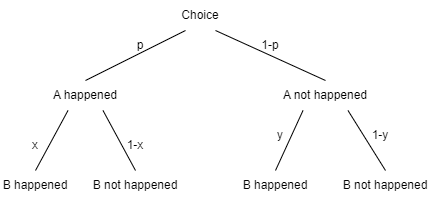
\includegraphics[scale=0.8]{independence.png}
    \end{figure}

    We define the paths of the graph as the independence decomposition of a complex events, providing a focus on particular situations. The probability value $x$ and $y$ are called conditional proability, which is a particular probaility of a given condition. We denote $P(B|A)=x$ to be the probability of $B$ when $A$ is given happening. Similarly, $P(B'|A)=1-x$ to be the probability of B does not happen when $A$ is given happening. $P(B|A')=y$ and $P(B'|A')=1-y$ for similar reasoning.

    In particular, we may observe that $px=P(A\cap B)$, and that becomes one of the formula defining conditional proability:

    \begin{theorem}
        Given $A$ and $B$ be two events, the conditional probability of $B$ given $A$ is happened is \[P(B|A)=\frac{P(A\cap B)}{P(A)}\]
    \end{theorem}

    The formula provides an interesting connection for the bi-directional conditional probability formula:

    \begin{corollary}
        Given $A$ and $B$ be two events, the following holds: \[P(A)P(B|A)=P(B)P(A|B)\]
    \end{corollary}

    To resolve the proability of $B$, we shall see the collection of all event $B$ is from both $A$ happens or not, hence it is natural to write $P(B)=px+(1-p)y$, which is in other words the total probability formula.

    \begin{theorem}
        The total probability of event $B$ is given by, when $A$ and $B$ are dependent on each other, \[P(B)=\sum P(A_n\cap B)=\sum P(A_n)P(B|A_n)\] where $A=\bigcup A_n$.
    \end{theorem}

    \subsection{Discrete random variables}

    \subsubsection*{Finite domain and infinite domain}

    \subsubsection*{Mean and expected value}

    \subsubsection*{Standard deviation and variance}

    \subsection{Distributions}

    \subsubsection*{Binomial distribution}

    \subsubsection*{Geometric distribution}

    \subsubsection*{Poisson distribution}

    \subsubsection*{Normal distribution and Standard distribution}

    \subsection{Sampling}

    \subsubsection*{Point sampling}

    \subsubsection*{Central limit theorem}

    \subsubsection*{Confidence interval}

    \subsection{Challenging questions}

\end{document}